%%%%%%%%%%%%%%%%%%%%%%%%%%%%%%%%%%%%%%%%%%%%%%%%%%%%%%%%%%%%%%%%%%%%%%%%%%%%%%%%%%%%%%%%%%%%%
%Debut d'importation de tous les paquets nécéssaire.
\documentclass[12pt,a4paper]{report}
\usepackage[utf8]{inputenc}
\usepackage[french,english]{babel}
\usepackage[T1]{fontenc}
\usepackage{listingsutf8}
\usepackage{texments}
\usepackage{layout}
\usepackage[hidelinks]{hyperref}
\usepackage{graphicx}
\usepackage{color}
\usepackage{enumitem} %package permettant de géner le changement des enumeration
\usepackage{setspace}%package permettant de gérer les interlines entres les phrases.
\usepackage{lscape}%c'est un packet qui permet de gérer l'orientation des pages.
\usepackage{lastpage}%est un paquet permettant de ressortir le numero de la fin de notre page
\usepackage{amsmath,amsfonts}
%chargement du package fancy propre aux entête et au pieds de pag
\usepackage{fancyhdr}
\parindent=0cm
%\usepackage{array}%c'est un packet permettant d'insérer un tableau dans un document latex
\usepackage{setspace}%commande permettant de gérer les interlines 
\usepackage[top=3cm, bottom=3cm, left=3cm, right=3cm]{geometry} 
\usepackage{lastpage}
\usepackage{tikz}%package permettant d'avoir la bordure de la prémiere de couverture
\usetikzlibrary{calc}%package pour la bordure de couverture
\newlength{\drop}
%Chargment de packages pour plusieurs types de letrines
\usepackage{lettrine,oldgerm,yfonts}
\usepackage{lipsum}
%fin d'importation des paquets
%doublespacing
%\onehalfspacing
%\setstretch{1.5}
%\renewcommand{\baselinestretch}{1.5} a placer avant le \begin{document}
%%%%%%%%%%%%%%%%%%%%%%%%%%%%%%%%%%%%%%%%%%%%%%%%%%%%%%%%%%%%%%%%%%%%%%%%%%%%%%%%%%%%%%%%%%%%%%%



%%%%%%%%%%%%%%%%%%%%%%%%%%%%%%%%%%%%%%%%%%%%%%%%%%%%%%%%%%%%%%%%%%%%%%%%%%%%%%%%%%%%%%%%%%%%%%%
%bloc de commande permettant de définir l'entête et le pied de page:
\lhead{}
\chead{\small{PRESENTATION DES 10 NORMES SUR LES CARTES A PUCE}}
\rhead{}

%bloc de commande permettant de définir le pied de page:
\lfoot{\small{Oumar Djimé RATOU}}
\cfoot{}
\rfoot{\thepage /\pageref{LastPage}}%commande permettant de reférencé le nombre total de page

%definissons la largeur de la ligne horizontale a l'entête de la page
\renewcommand{\headrulewidth}{2pt}
%definissons la largeur de la ligne horizontale a l'entête de la page
\renewcommand{\footrulewidth}{2pt}
%%%%%%%%%%%%%%%%%%%%%%%%%%%%%%%%%%%%%%%%%%%%%%%%%%%%%%%%%%%%%%%%%%%%%%%%%%%%%%%%%%%%%%%%%%%%%%%


%\renewcommand{\thepart}{\Roman{part}}
%.\arabic{subsection}.\roman{subsubsection}}
%%%%%%%%%%%%%%%%%%%%%%%%%%%%%%%%%%%%%%%%%%%%%%%%%%%%%%%%%%%%%%%%%%%%%%%%%%%%%%%%%%%%%%%%%%%%%%%
%présentation de la prémière de couverture
\begin{document}
%\maketitle

%\selectlanguage{french}
\begin{tikzpicture}[remember picture, overlay]
	\draw[line width = 2pt] ($(current page.north west) + (1.75cm,-1.75cm)$) rectangle ($(current page.south east) + (-1.75cm,1.75cm)$);
\end{tikzpicture}
\thispagestyle{empty}
\pagenumbering{roman}
%\selectlanguage{francais}
%nous activons la numerotation roman
%debut page de garde
\begin{minipage}[c]{.35\textwidth}
%	\center
    \footnotesize
    \begin{center}
    République du Cameroun\\
	****\\
	Paix-Travail-Patrie\\
	****\\
	Ministère de l’Enseignement Supérieur\\
	****\\
	Université de Maroua\\
	****\\
	Ecole Nationale Supérieure Polytechnique de Maroua\\
    \end{center}
\end{minipage}
\begin{minipage}[c]{.3\textwidth}
	\begin{center}
		
\includegraphics[scale=0.4]{univ.png}
	\end{center}
\end{minipage}
\begin{minipage}[c]{.35\textwidth}
%    \center
    \footnotesize
    \begin{center}
    Republic of Cameroon\\
	****\\
	Peace-Work-Fatherland\\
	****\\
	Ministry of Higher Education\\
	****\\
	The University of Maroua\\
	****\\
	The Polytechnic National Advanced School of Maroua\\
    \end{center}
\end{minipage}
%fin page de garde
%titre du thème
\begin{center}
	\drop=0.07\textheight %commande permettant de gerer la l'espace entre deux texte
	\vspace{0.5\drop}
	INFORMATIQUE ET TELECOMMUNICATIONS\\
	\drop=0.07\textheight 
	\vspace{0.4\drop}
	\textbf{CRYPTOGRAPHIE ET SÉCURITÉ INFORMATIQUE}
	\rule{.95\textwidth}{2pt}\\
	\large{\textbf{PRESENTATION DES 10 NORMES SUR LES CARTES A PUCE}}\\
	\rule{.95\textwidth}{2pt}\\%commande permettant de désigné un trait horizontal de longueur .95 et de 			largeur 2pt

\end{center}


\begin{center}
	%\drop=0.07\textheight %commande permettant de gerer la l'espace entre deux texte
	%\vspace{0.2cm}
	\textbf{Mémoire présenté et soutenu en vue de l’obtention du Diplôme}\\
	\vspace{0.2cm}
	\textbf{D’INGÉNIEUR DE CONCEPTION EN CRYPTOGRAPHIE ET SÉCURITÉ INFORMATIQUE}\\
	\vspace{0.2cm}
	Par \\
	\vspace{0.2cm}
	\textbf{OUMAR DJIMÉ RATOU}\\
	\vspace{0.2cm}
	\textbf{Matricule : 17Y402P}\\
	\vspace{0.3cm}
	Sous la Direction de : \\
	\vspace{0.2cm}
	\textbf{Dr. KALADZAVI GUIDEDI}\\
	\vspace{0.2cm}
	Chargé de Cours
	
	

\end{center}


	
\drop=0.8\textheight%commande nous permettant de définir la l'espace entre deux paragraphes
\vspace{0.1\drop}%commande nous permettant de définir la l'espace entre deux paragraphes
\begin{center}
	
	
	Devant le jury composé de :\\
	\vspace{0.2cm}
	\emph{\textbf{Président : }}  \textit{M. LAOUKOURA Charles}\\
	\emph{\textbf{Rapporteur : }}  \textit{M. LAOUKOURA Charles}\\
	\emph{\textbf{Examinateur : }}  \textit{M. LAOUKOURA Charles}\\
	
	\drop=0.2\textheight%commande nous permettant de définir la l'espace entre deux paragraphes
	\vspace{0.5\drop}
	\textit{ANNÉE ACADÉMIQUE:} \textbf{2018/2019}
\end{center}
%\end{center}
%fin de la préssentation
%fin de présentation de la prémière de couverture
%%%%%%%%%%%%%%%%%%%%%%%%%%%%%%%%%%%%%%%%%%%%%%%%%%%%%%%%%%%%%%%%%%%%%%%%%%%%%%%%%%%%%%%%%%%%%%%%%



%%%%%%%%%%%%%%%%%%%%%%%%%%%%%%%%%%%%%%%%%%%%%%%%%%%%%%%%%%%%%%%%%%%%%%%%%%%%%%%%%%%%%%%%%%%%%%%%%
%debut du rapport
\onehalfspacing
\newpage

\setcounter{page}{1}

\newpage

%PArtie de dédicace
\section*{Dédicaces}

\pagebreak

%Partie de rémerciement
\section*{Remerciement}

\pagebreak

%Abstract francais
\selectlanguage{french}
%\renewcommand{\contentsname}{Sommaire} : commande permettant de remplacer table des matière en sommaire
%%%%%%%%%%%%%%%%%%%%
\tableofcontents   %
%%%%%%%%%%%%%%%%%%%%



\pagebreak
%Listees des abréviations
\section*{Listes des abréviations}

\pagebreak
%Résumé et abstract


%\setlength{\parindent}{0pt} %Supprime l'indentation de tous le document
\begin{abstract}
	\lipsum[2]
\end{abstract}
%Abstract anglais
\selectlanguage{english}
\begin{abstract}
	\lipsum[2]
\end{abstract}

%On repasse en francais pour la suite de texte
\selectlanguage{french}

% Mot clés
\section*{Keyswords ou mot clé}

\pagebreak
% Listes de tableau
\section*{Liste des tableaux}

\pagebreak

% Listes de figures et illustration
\section*{Listes de figures et illustration}

%\pagenumbering{roman}
\newpage 	
\pagenumbering{arabic}		
\pagestyle{fancy}
%corps du rapport
%\begin{flushleft}


\newpage
%Introduction général
\addcontentsline{toc}{section}{Introduction}
\section*{Introduction}
\newpage

%Premier partie
\part{Présentation générale}


% Chapitre 1 contexte et problematique
%\chapter{Contexte et problématique}

	\addcontentsline{toc}{section}{Introduction}
	\section*{Introduction}
	\lettrine{D}{ans} ce chapitre de la première partie, nous présentons l'entreprise où nous avons effectué notre stage académique à savoir ITS GROUP. Nous parlerons ensuite du contexte relatif à notre sujet de stage de fin d'étude, nous terminerons par une mise en évidence de la problématique lié à ce contexte  et les objectifs à atteindre. 
	

	%Presentation de l'entreprise
	\section{Présentation de l'entreprise}
		\subsection{Historique}
			ITS GROUP est une entreprise en sécurité de système d'informations de droit camerounais dont le siège générale se trouve à Yaoundé(BP...)
		
		\subsection{Organisation générale}
		
		
		\subsection{Missions}
		
		\subsection{Services et Produits}
		
		\subsection{Cadre de stage}
		
			\subsubsection{Situation géographique}
			
	\section{Contexte}
	
	\section{Problématique}
	
	\section{Objectifs}
	
		\subsection{Objectif général}
		
		\subsection{Objectif spécifique}
		
	\section{Méthodologie}
	
	%\addcontentsline{toc}{section}{Conclusion}
	\section*{Conclusion}

\chapter{Contexte et problématique}

	\addcontentsline{toc}{section}{Introduction}
	\section*{Introduction}
	\lettrine{D}{ans} ce chapitre de la première partie, nous présentons l'entreprise où nous avons effectué notre stage académique à savoir ITS GROUP. Nous parlerons ensuite du contexte relatif à notre sujet de stage de fin d'étude, nous terminerons par une mise en évidence de la problématique lié à ce contexte  et les objectifs à atteindre. 
	

	%Presentation de l'entreprise
	\section{Présentation de l'entreprise}
		\subsection{Historique}
			ITS GROUP est une entreprise en sécurité de système d'informations de droit camerounais dont le siège générale se trouve à Yaoundé(BP...)
		
		\subsection{Organisation générale}
		
		
		\subsection{Missions}
		
		\subsection{Services et Produits}
		
		\subsection{Cadre de stage}
		
			\subsubsection{Situation géographique}
			
	\section{Contexte}
	
	\section{Problématique}
	
	\section{Objectifs}
	
		\subsection{Objectif général}
		
		\subsection{Objectif spécifique}
		
	\section{Méthodologie}
	
	%\addcontentsline{toc}{section}{Conclusion}
	\section*{Conclusion}


% Chapitre 2 
\chapter{Généralités sur la signature électronique et PKI }
	\section*{Introduction}
	
	\section{Généralités sur la signature électronique}
		\subsection{Signature électronique}
			\subsubsection{Définitions}
			\subsubsection{Rôle de signature électronique}
	\section{Cryptographie}
		\subsection{Cryptographie symétrique}
		\subsection{Cryptographie asymétrique}
	
	\section{Infrastructure à clé publique}
	
			
\section*{Conclusion}



%Premier partie
\part{Conception et test}

%Chapitre 3
\chapter{Analyse, Conception et déploiement du module}

	\section*{Introduction}
		Une fois que la présentation des concepts liée à notre projet est faite, nous allons effectuer l'analyse et la conception de notre module de signature électronique. Pour cela, nous effectuerons premièrement le choix de cycle de vie de développement d'un logiciel qui nous convient, deuxièmement nous procéderons à l'analyse de besoins, ensuite nous ferons la conception proprement dite et enfin nous terminerons par l'implémentation du système.
	
	\section{Choix du cycle de développement}
		Le cycle de vie d'un logiciel indique les étapes par lesquelles doit passer un logiciel de sa conception jusqu'à sa mort. Ce cycle de vie permet de détecter les erreurs tout au long du processus de réalisation et ainsi les corriger pour produire un logiciel de qualité, maîtriser les délais de sa réalisation et les coûts associés.
		Le cycle de vie d'un logiciel comprend généralement les étapes suivantes:
		\begin{enumerate}
			\item \textbf{Pré-étude :} Cette étape permet de définir les objectifs du projet de définir le domaine d'activité. Les questions poser sont :\textbf{Quoi?, Combien? et Quoi?}
			
			\textit{En entrée, on a les besoins et en sortie on a un cahier de charges.}
			\item \textbf{Analyse : } Cette consiste à recueillir les informations et formaliser les besoins du client, de définir les contraintes et d'estimer la faisabilité de ce besoins. La question à poser est : \textbf{que fait le système?}
			
			\textit{En entré, on a le cahier de charge et en sortie on a le dossier d'analyse.}
			
			\item \textbf{Conception :} Cette étape permet d'élaborer la structure générale du système et de définir chaque sous-ensemble de logiciel à produire. La question à poser est : \textbf{comment faire ce qu'il est demandé de faire ?}
			
			\textit{En entré, on a le dossier d'analyse et en sortie on a un dossier de conception.}
			\item \textbf{Codage : }Cette étape consiste à coder ou à programmer les fonctionnalités définis dans la phase de conception.
			
			\textit{En entré, on a le dossier de conception en sortie on a des programmes.}
			\item \textbf{Tests : }Cette étape permet de tester le logiciel conformément aux spécifications(fonctionnelle ou non fonctionnelle). Il existe quatre types de tests à savoir :\textbf{ le test unitaire, le test d'intégration, le test fonctionnel et le test de validation.}
			
			\item \textbf{Réception : } Cette étape permet au client de vérifier la conformité de logiciel avec les spécifications initiales.
			
			\textit{En entré on a un logiciel plus un cahier de charge et en sortie on a un procès verbal de réception\textbf{(acception ou refus du livrable)}}.
			
			\item \textbf{Maintenance : } Cette étape permet de prendre en charge les actions collectives du système\textbf{(Maintenance collective et évolutive).}
			
			En entré on a un logiciel et en sortie on a un logiciel modifié.
					\end{enumerate}
					
			Nous avons vu quelles sont les étapes clés dans le cycle de vie d'une 	application. Afin d'obtenir un résultat optimal, il est conseillé de suivre cette démarche qui peut subir des améliorations\cite{suppinfo}.
			
			Il existe plusieurs modèles de cycle de vie à savoir : le cycle en cascade, le cycle en V, le cycle en spirale, le cycle semi-itératif mais dans notre cas on a décider de suivre le modèle du cycle en V.
			\begin{figure}[H]
					\centering		
					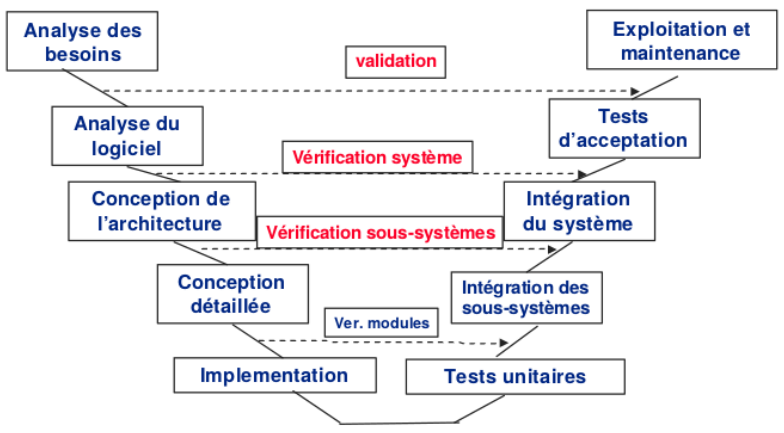
\includegraphics[width=18cm, height=8cm]{../imgs/v.png} 				
					\caption{Modèle de cycle en V}
					\label{fig3}
			\end{figure}
			
			\subsubsection{Pourquoi cycle en V ?}
			% description de modele choisi
			Il est introduit en \textbf{1997}. La version actuelle est désignée de \textbf{V-Modell XT}(depuis février 2005). Cette méthode consiste en un modèle  pour la planification et le développement de logiciel\cite{kolyang}. Le modèle V répond à quatre requête importantes de développement: \textbf{Who? What? When? How?}
			
			L'on peut poser la question comme suit: \textbf{Who has to do what, when, and how whithin a project?} \textbf{Qui doit faire quoi, quand et comment dans un projet ? }Cette question est capital lors de la construction d'un logiciel.
			
			Par ailleurs, dans le modèle V, le fond réalise l'implémentation. La branche gauche définit les différentes spécifications. La branche droite crée des corrélations avec la partie gauche à savoir la validation du système, la vérification système et du logiciel.
			
			L'accent est mis sur la réduction des erreurs. La branche droite permet en général la détection rapide des erreurs et des anomalies présents dans la partie gauche et entreprend des mesures adéquates pour les corriger. Et en plus, la finalité de cycle de vie en V consiste à parvenir sans incident à livrer un logiciel totalement conforme au cahier des charges\cite{kolyang}. Voila pourquoi nous avons choisi le modèle V.
			
	\section{Orientation et faisabilité}
		Le projet intitulé  \og Conception et déploiement d'un module de signature numérique basé sur l'architecture à clé  publique \fg  est né  du fait que l'entreprise ITS à constater qu'il n'y a pas un module de signature électronique disponible pour les développeurs pour intégrer dans leurs plate-formes en général et un système de complet de signature électronique libre et transparent en particulier.
		
		Par ailleurs, bien qu'ils existent des tels  systèmes tels que  Word de Microsoft et Adobe Reader mais ne sont pas dans les systèmes d’exploitation libre(open source) comme Linux.
		
	Les problèmes qui surviennent souvent dans les entreprises en particulier et chez les développeurs en général c’est la disposition des programmes modulaires pour intégrer facilement dans leurs plates-formes en fin de gagner en temps et en l’argent (surtout pour les entreprises).
	
	L’environnement dans lequel nous nous trouvons est favorable au projet puisqu’un tel système existe certes mais sous une licence payante et non modulable. Sa mise en œuvre sera une innovation importante dans l’évolution numérique au sein de l’entreprise et dans le monde de open source.
	
	L'utilisation du système bénéficiera à ITS de :
	\begin{itemize}
		\item Signer désormais ces documents numériques,
		\item Utiliser le module dans un projet de même thématique facilement,
		\item permet d'avoir son propre outil de signature électronique.\\
	\end{itemize}

Ce projet d'inscrit donc largement dans le cadre de la sécurité de système d'information qui est aujourd’hui très capital tant pour les entreprises que les utilisateurs. 



	\section{Analyse de besoins }
		Dans cette section, nous allons recueillir les besoins du demandeur (le client) et l'ensemble des contraintes liés au système à mettre sur pied.
		\subsection{Cahier de charge}
			Le cahier de charge a pour but de présenter notre projet su la signature électronique basé sur l'architecture à clé publique des documents numériques de l'entreprise ITS et autres tel que spécifié dans la section précédente.
		\subsubsection{Besoins fonctionnels}
			Il est question ici de présenter toutes les fonctionnalités du système. Ce sont les besoins spécifiant un comportement d'entré/sortie du système. Le système doit permettre à :
			\begin{enumerate}
				\item l'Administrateur de :
					\begin{itemize}
						\item  gérer les comptes (supprimer, modifier, bloquer etc),
						\item  générer une paire de clé(publique et privée),
						\item  signer un document numérique à l’aide de la clé privée,
						\item  générer un certificat (auto-signé, puisque le signé est payant),
						\item  vérifier la signature d’un document numérique à l’aide de la clé publique,
						\item  chiffrer/déchiffrer un document,
						\item  générer un Hash du document numérique.
					\end{itemize}
					Il faut noter que l'administrateur ne pourra effectuer ces fonctionnalités que s'il est authentifier avec son compte administrateur, question de sécurité.
				\item l'Utilisateur de:
						\begin{itemize}
						\item  générer une paire de clé(publique et privée),
						\item  signer un document numérique à l’aide de la clé privée,
						\item  générer un certificat (auto-signé, puisque le signé est payant),
						\item  vérifier la signature d’un document numérique à l’aide de la clé publique,
						\item  chiffrer/déchiffrer un document,
						\item  générer un Hash du document numérique.
					\end{itemize}
				\item au système externe de :
						\begin{itemize}
						\item  générer une paire de clé(publique et privée),
						\item  signer un document numérique à l’aide de la clé privée,
						\item  générer un certificat (auto-signé, puisque le signé est payant),
						\item  vérifier la signature d’un document numérique à l’aide de la clé publique,
						\item  chiffrer/déchiffrer un document,
						\item  générer un Hash du document numérique.
					\end{itemize}
			\end{enumerate}
			
		\subsubsection{Besoins non fonctionnels}
			A part les besoins fondamentaux, notre système doit répondre aux critère suivants :
				\begin{itemize}
					\item la rapidité de traitement :  En effet, vu le nombre important des transactions quotidiennes, il est impérativement nécessaire que la durée d'exécution des traitements s'approche le plus possible du temps réel;
					\item la performance: Un logiciel doit être avant tout performant c'est-à-dire à travers ses fonctionnalités, répond à toutes les exigences des usagers d'une manière optimale;
					\item La convivialité : Le futur logiciel doit être facile à utiliser. En effet, les interfaces utilisateurs doivent être conviviales c'est-à-dire simples, ergonomiques et adaptées à l'utilisateur.
				\end{itemize}
				Elle devra aussi être capable de :
				\begin{itemize}
					\item tourner en réseaux pour qu'il soit accessible de tous,
					\item être compatible avec n'importe quel système d'exploitation, smartphone, tablette et OS.
					
				\end{itemize}
				
					Il faut aussi souligner que l'application devra être hautement sécurisé car les informations ne devront pas être accessible de tous, sauf pour les légitimes.
					
	\section{ Budgétisation}
	\begin{minipage}{\textwidth}
		
			\begin{center}
				\definecolor{gris1}{gray}{0.85}
				\definecolor{gris2}{gray}{0.85}
			\begin{tabular}{|l|*{4}{c|}}
				\hline
					{Ressources}&Noms&Quantité&Prix unitaire &Total\\ 
				\hline
				\rowcolor{gris1}Tétraèdre&4&6&4&4+4-6=2\\ \hline
				Cube&8&12&6&\cellcolor{gris2}8+6-12=2\\ \hline	
			\end{tabular}
		\end{center}
	\end{minipage}
	
	\section{Conception architecturale}
		Nous élaborons les spécifications de notre architecture générale de notre système. Nous optons pour une architecture client serveur centralisée. L'environnement client/serveur désigne un mode de communication organisé par l'intermédiaire d'un réseau et d'un interface Web entre plusieurs ordinateurs . \og cela signifie que des machines clientes (machines faisant partie du réseau) contactent un serveur, une machine généralement très puissante en terme de capacités d'entrées-sorties , qui leur fournit des services. Lesquels services sont exploités par des programmes ,appelés programmes clients, s'exécutant sur les machines clientes. \fg
		
		Puisqu'il existe plusieurs environnements client/serveur(Architecture "\textbf{Peer to Peer}",Architecture à 2 niveaux,Architecture à 3 niveaux, etc), plus précisément nous optons pour une architecture client/serveur Peer to Peer. Le réseau est dit pair à pair (peer-to-peer en anglais, ou P2P), lorsque chaque terminal connecté au réseau est susceptible de jouer tour à tour le rôle de client et celui de serveur.
		
			\begin{figure}[H]
					\centering		
					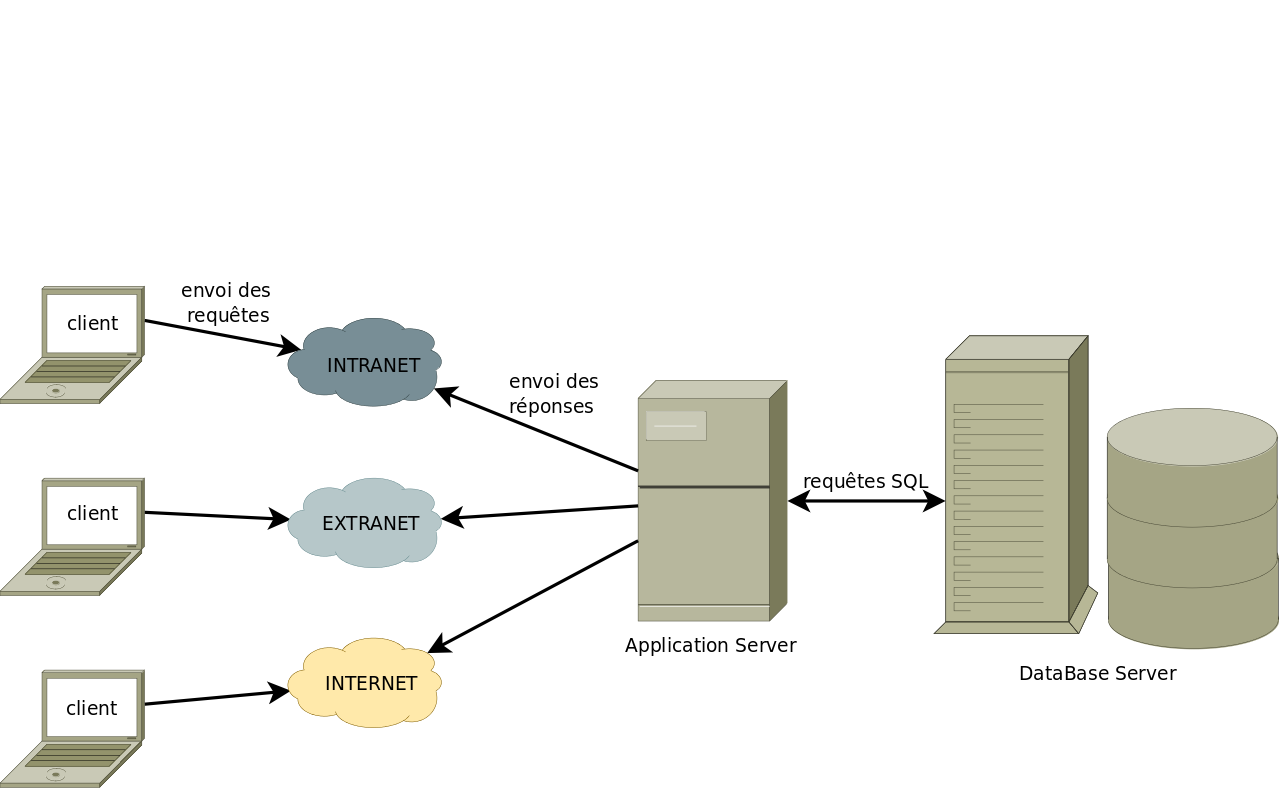
\includegraphics[width=18cm, height=13cm]{../imgs/clientserveur.png} 				
					\caption{Architecture Client Serveur }
					\label{archiclientserver}
			\end{figure}
		
		
	
	\section{Conception détaillée}
		Pour réaliser la conception détaillée de notre système nous utiliserons le langage de modélisation UML (Unified Modeling Language).
		\subsection{Présentation de langage UML}
			L'UML (pour Unified Modeling Language, ou "langage de modélisation unifié" en français) est un langage permettant de modéliser nos classes et leurs interactions. Autrement c’est un ensemble de notations graphiques s’appuyant sur des diagrammes et permettant de spécifier, visualiser et de documenter les systèmes logiciels orientés-objet. UML utilise des diagrammes pour modéliser un système. Il ne s’agit pas d’une simple notation graphique car les concepts transmis par un diagramme ont une sémantique\cite{SMSSEC}.

	En ce qui concerne la structure du formalisme UML, il peut être vu comme nous montre la figure suivante:
			\begin{figure}[H]
					\centering		
					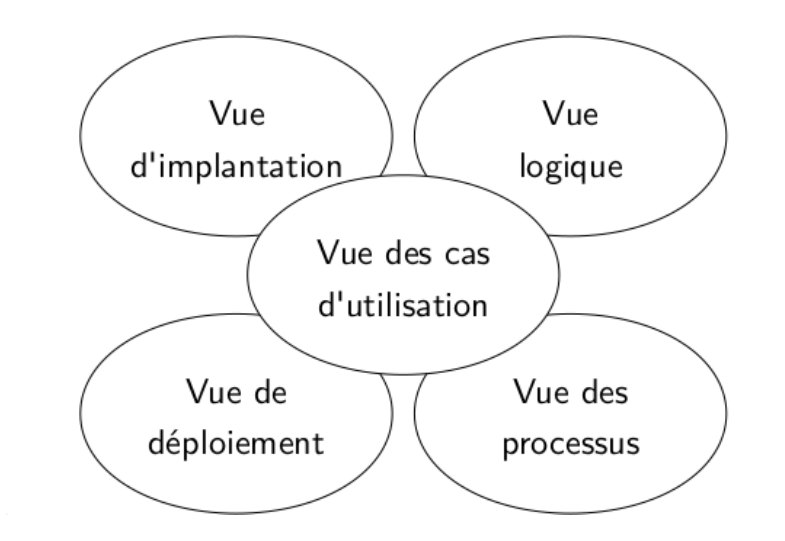
\includegraphics[width=18cm, height=13cm]{../imgs/uml.png} 				
					\caption{différentes vues du formalisme UML }
					\label{vueuml}
			\end{figure}
			
		A chaque vue est associée certains diagramme :
		\begin{itemize}
			\item \textbf{ Vue de cas d'utilisation\cite{opensclass1} :}  S'applique à l'ensemble des cas d'utilisation qui décrivent ensemble le comportement d'un système donné vu par ses acteurs. Cette vue indique les forces internes et externes qui forment l'architecture du système. Elle définit les besoins des clients du système et centre la définition de l'architecture du système sur la réalisation de ces besoins ; elle conduit à la définition d'un modèle d'architecture pertinent et cohérent en se basant sur les scénarios décrits dans les cas d’utilisation.
			
Elle motive les choix, permet d'identifier les interfaces critiques et force à se concentrer sur les problèmes importants.
			\item \textbf{Vue logique : } a pour but d’identifier les éléments du domaine, les relations et interactions entre ces éléments. Cette vue organise les éléments du domaine en « catégories ». Deux diagrammes peuvent être utilisés pour cette vue : diagramme de classes et diagramme des objets.
			\item \textbf{Vue des processus :} Démontre la décomposition système en processus et actions, les interactions entres les processus, la synchronisation et la communication des activités parallèles. Elle s'appuie sur plusieurs diagrammes : diagramme de séquence, diagramme d'activité, diagramme de collaboration etc.
			\item \textbf{Vue de déploiement :} décrit les ressources matérielles et la répartition des parties du logiciel sur ces éléments. Il contient un diagramme : le diagramme de déploiement.
			
			\item \textbf{Vue d'implémentation :} Décrit l'ensemble des algorithmes utilisés et le code source\cite{opensclass1}.


		\end{itemize}
		
		\subsection{Modélisation avec le langage UML}
		Pour modéliser notre système avec le langage UML, nous allons utiliser les outils suivants :
		\begin{enumerate}
			\item Astah-pro, version d'évaluation,
			\item Umbrello,
			\item GIMP 2.10.
		\end{enumerate}
			
			\subsubsection{Diagramme de cas d'utilisation}
				Le diagramme des cas d’utilisation est une notation très simple et compréhensible par tous et qui permet de structurer les besoins (cahier des charges) et le reste du développement. Un diagramme de cas d’utilisation décrit les acteurs\footnote{ Un acteur est un utilisateur, humain ou non, du système qui est doté d’un nom qui correspond à son rôle.}, les cas d’utilisation\footnote{Un cas d’utilisation est une manière spécifique d’utiliser le système.} et le système. Un modèle de cas
utilisation peut être formé de plusieurs diagrammes de cas d'utilisation, de descriptions textuelles, de diagrammes de séquences. Un cas d’utilisation CU) décrit une manière d’utiliser le système en une suite d’interactions entre un acteur et le système.
				\begin{enumerate}
					\item \textbf{Diagramme de cas d'utilisation général :}
						\begin{figure}[H]
						\centering		
							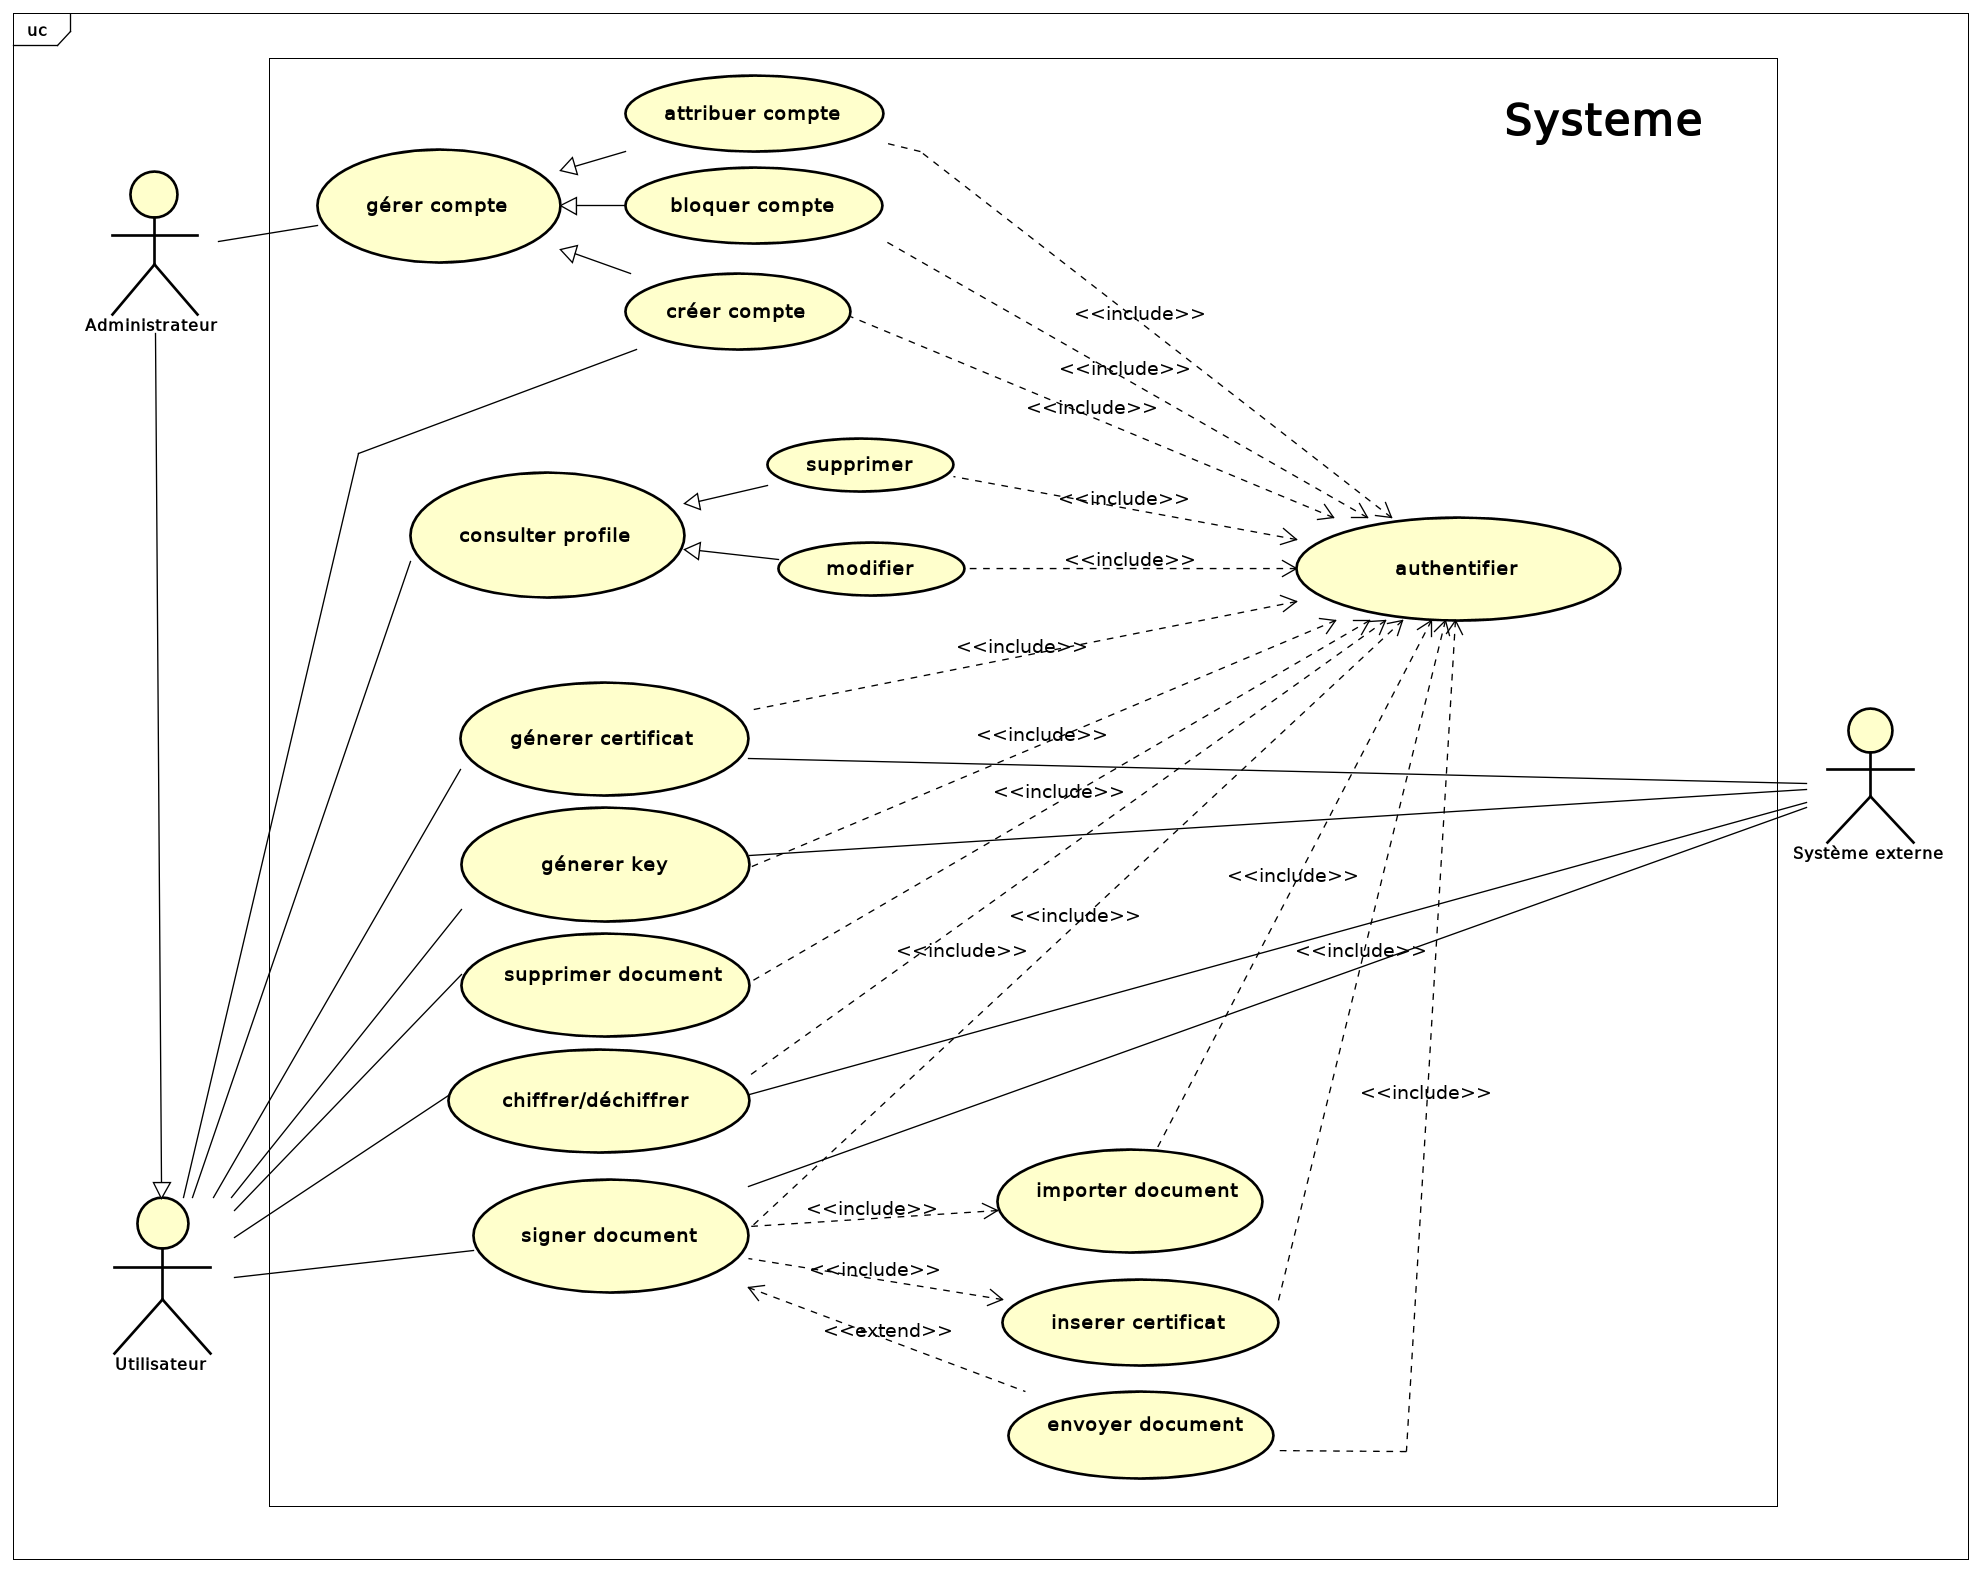
\includegraphics[width=18cm, height=13cm]{../Diagrammes/DiagrammeDeCasDutilisation/diagrammeGeneral.png} 
						\caption{Diagramme de cas d'utilisation général}
						\label{diause1}
					\end{figure}
					\item \textbf{Diagramme de cas d'utilisation de l'administrateur :}
					\begin{figure}[H]
						\centering		
						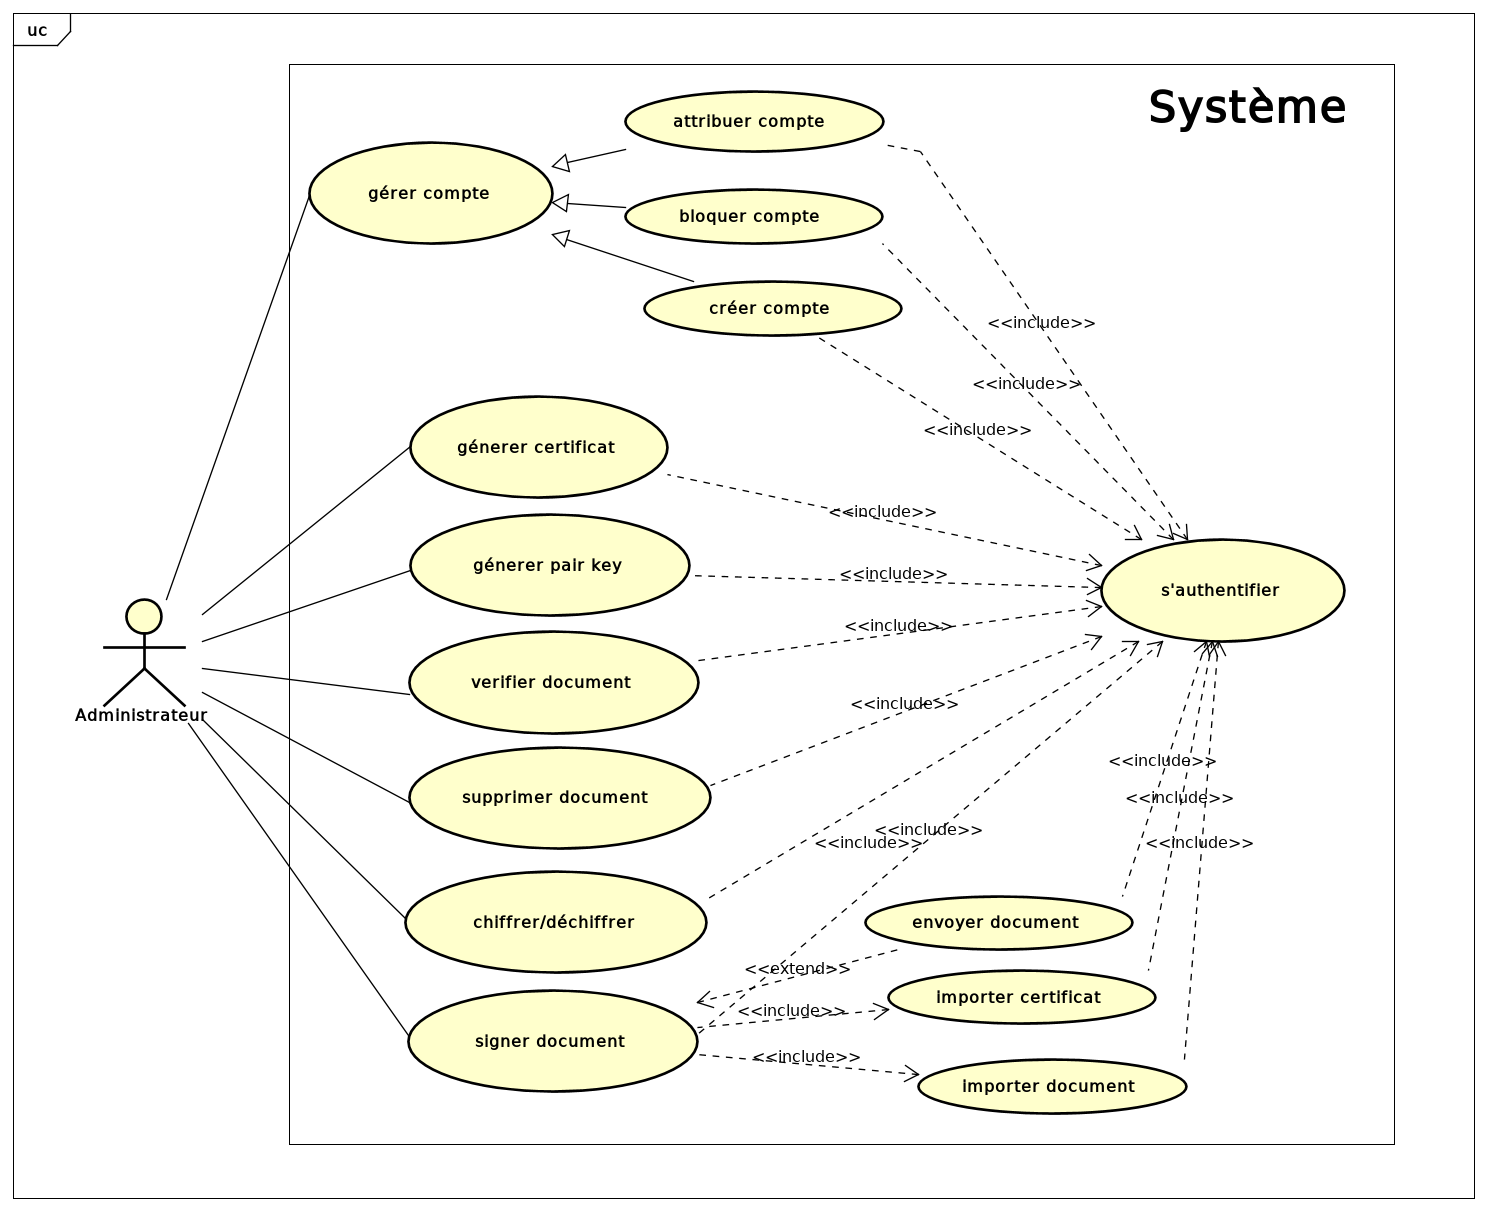
\includegraphics[width=18cm, height=13cm]{../Diagrammes/DiagrammeDeCasDutilisation/admin.png}  
						\caption{Diagramme de cas d'utilisation d'administrateur}
						\label{diause2}
					\end{figure}
					
					\item \textbf{Diagramme de cas d'utilisation de l'utilisateur :}
					\begin{figure}[H]
						\centering		
						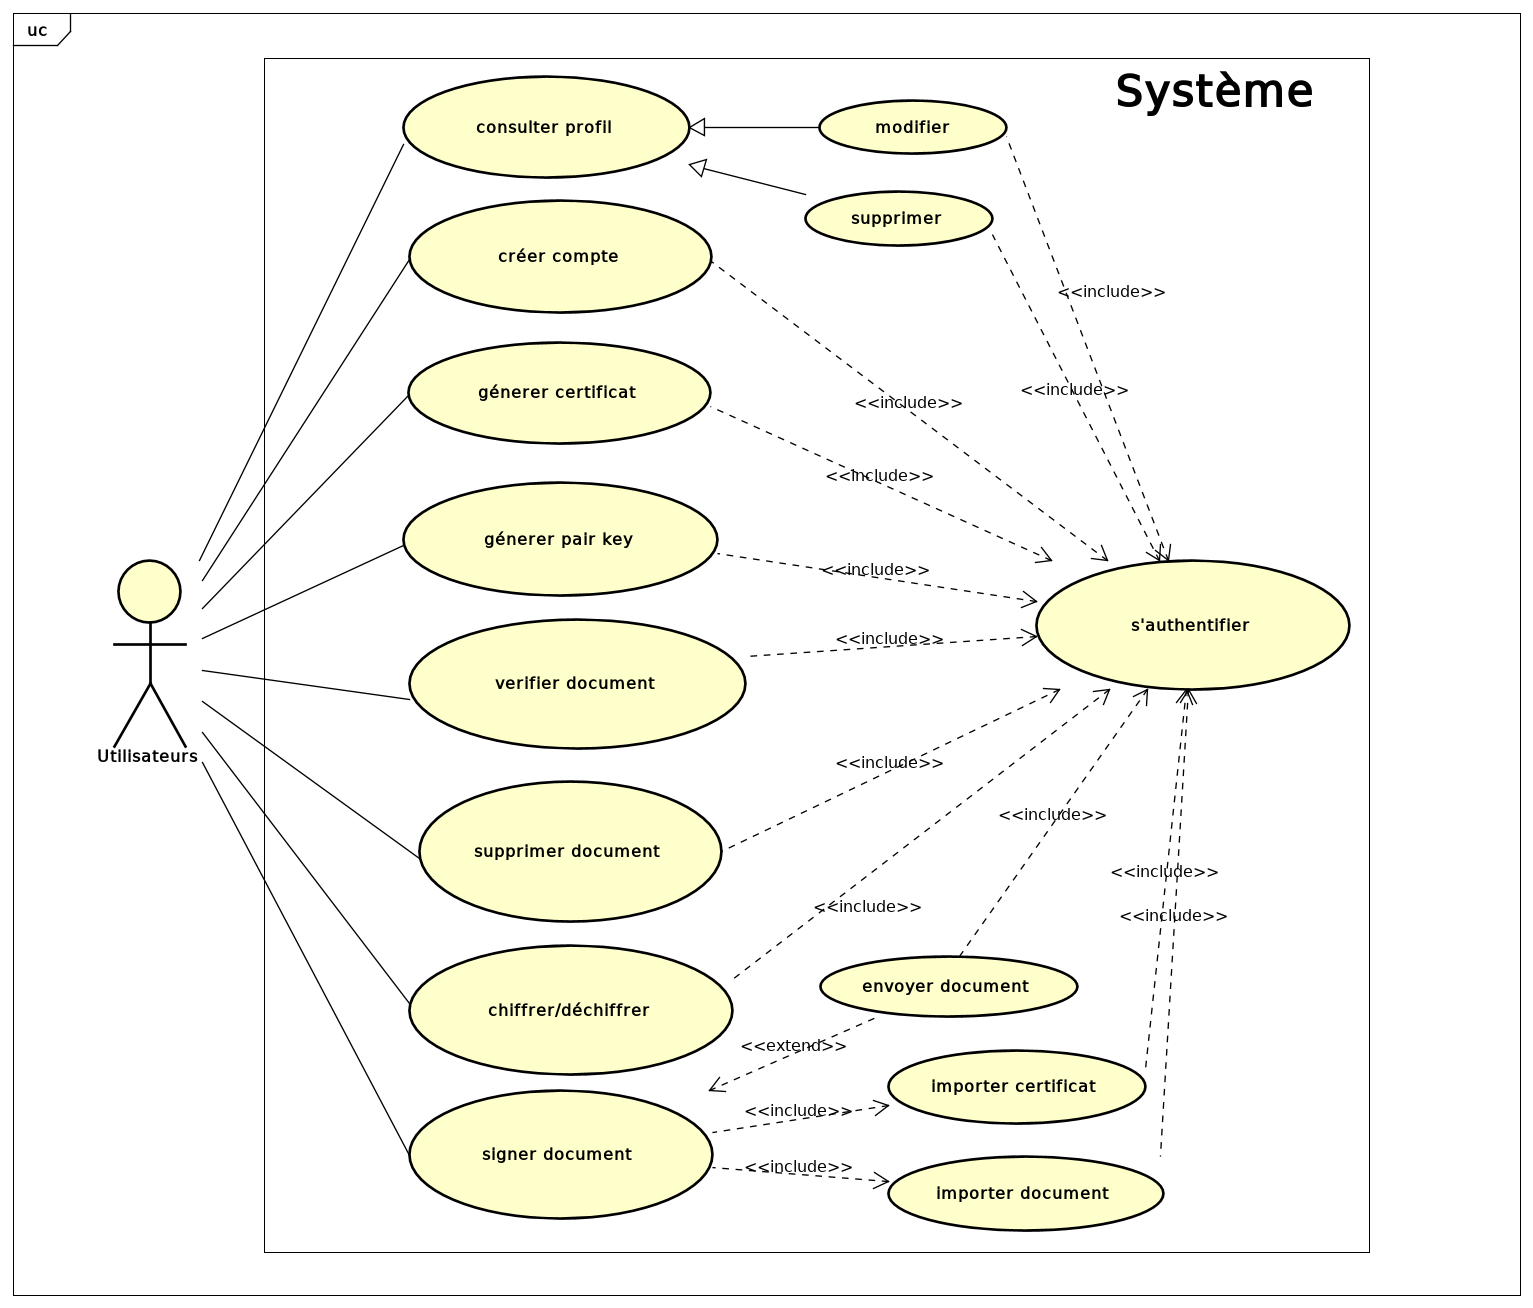
\includegraphics[width=18cm, height=13cm]{../Diagrammes/DiagrammeDeCasDutilisation/users.png}  
						\caption{Diagramme de cas d'utilisation d'utilisateur}
						\label{diause3}
					\end{figure}
					
					\item \textbf{Diagramme de cas d'utilisation de système externe :}
						\begin{figure}[H]
							\centering		
							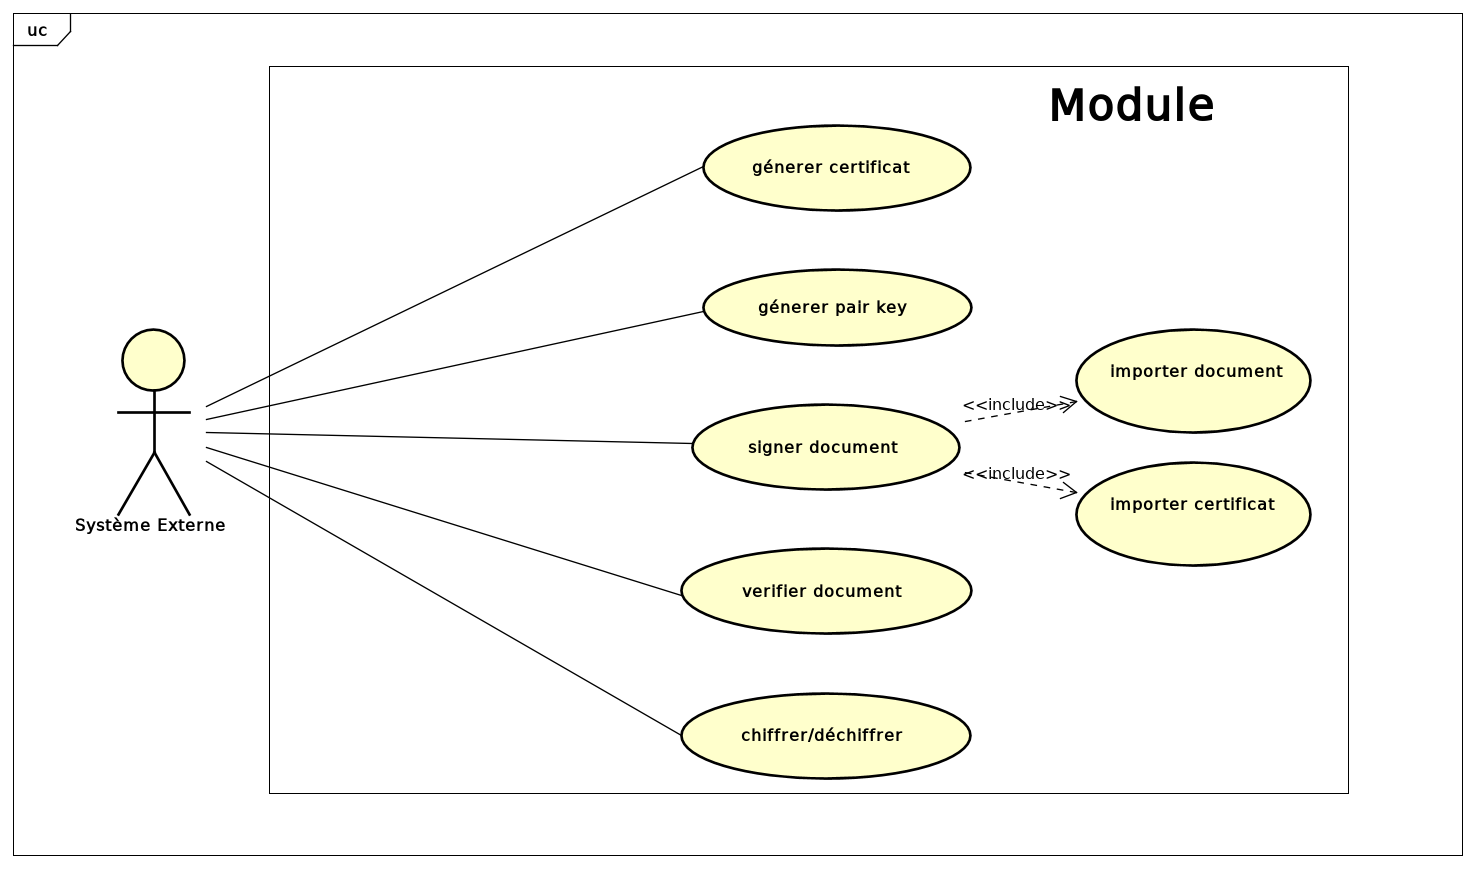
\includegraphics[width=18cm, height=13cm]{../Diagrammes/DiagrammeDeCasDutilisation/sysexterne.png}  
							\caption{Diagramme de cas d'utilisation de système externe}
							\label{diause4}
						\end{figure}
			
				\end{enumerate}
				
				\subsubsection{Description textuelle}
					\begin{enumerate}
						\item Description textuelle de cas d'utilisation : \textbf{S'authentifier}
							\begin{table}[H]
								\centering
								\caption{Description contextuelle de cas d'utilisation s'authentifier}
								\begin{tabular}{|l|p{11cm}|}
								\hline 
									\textbf{Titre} & S'authentifier \\ 
								\hline 
									\textbf{Résumé} & Ce cas d'utilisation permet d'accéder au tableau de bord de l'utilisateur \\ 
								\hline 
									\textbf{Acteur} & Administrateur, utilisateur \\  
								\hline 
									\textbf{Pré-condition} & l'application doit être lancer(page d'accueil) \\ 
								\hline 
								\multirow{2}{*}{\textbf{Scenario nominal}} & 1) l'utilisateur fait une demande l'accès au système en cliquant sur le bouton connexion, \\
							 & 2) le système lui renvoi le formulaire de connexion \\
							 & 3) l'utilisateur introduit son username et password \\
							 & 4) le système vérifie que  sont username et password corrects \\
							 & 5) le système ouvre une session de l'utilisateur \\
							\hline 
								\multirow{2}{*}{\textbf{Enchaînement Alternatif}} & le username et le password sont corrects., \\
							    & l'enchaînement commence au point 3 du scénario nominal. \\
							    & le message affiche un message d'erreur, aller au point 2. \\
							\hline 
								\textbf{Enchaînement d'Erreur} & E1 : Si l'étape 2 de scenario nominal n'est pas vérifié un message d'erreur sera affiché. \\
							\hline
								\textbf{Post condition} & ouverture d'une session, accès au compte\\
							\hline
						\end{tabular} 
					\end{table}
		
					\item Description textuelle de cas d'utilisation : \textbf{Générer certificat} 
					
					\begin{table}[H]
			
					\centering
					\caption{Description contextuelle de cas d'utilisation générer certificat}
					\begin{tabular}{|l|p{11cm}|}
					\hline 
						\textbf{Titre} & Générer Certificat \\ 
					\hline 
						\textbf{Résumé} & Ce cas d'utilisation permet de générer des certificats aux utilisateurs \\ 
					\hline 
						\textbf{Acteur} & Autorité de certification Administrateur, Système externe \\  
				
					\hline 
						\textbf{Pré-condition} & l'application doit être lancer (page d'accueil) \\ 
					\hline 
						\multirow{2}{*}{\textbf{Scenario nominal}} & 1) un AC peut générer un certificat en cliquant sur le bouton genererCertifcat, \\
							 & 2) le système lui renvoi le formulaire à remplir \\
							 & 3) on introduit la clé publique de l'utilisateur \\
							 & 4) on renseigne le nom et le prénom de l'utilisateur \\
							 & 5) la date de validité (début et fin)\\
							 & 6) numéro de version\\
							 &7) numéro de série. \\
					\hline 
					
						\multirow{2}{*}{\textbf{Enchaînement Alternatif}} & la clé publique n'est pas corrects. \\
							  & l'enchaînement commence au point 2 du scénario nominal. \\
							
					\hline 
						\textbf{Enchaînement d'Erreur} & E1 : Si l'étape 2 de scenario nominal n'est pas vérifié un message d'erreur sera affiché. \\
					\hline
						\textbf{Post condition} & création de certificat avec succès.\\
					\hline
			\end{tabular} 
		\end{table}
						\item Description textuelle de cas d'utilisation : \textbf{Générer Paire de Clé}
	
						\begin{table}[H]
			
						\centering
							\caption{Description contextuelle de cas d'utilisation générer paire de clé}
						\begin{tabular}{|l|p{11cm}|}
						\hline 
						\textbf{Titre} & Générer Paire de clé \\ 
						\hline 
						\textbf{Résumé} & Ce cas d'utilisation permet de générer des paires de clé aux utilisateurs \\ 
						\hline 
						\textbf{Acteur} & Autorité de certification, Administrateur, Système externe, Utilisateur \\  
						\hline 
						\textbf{Pré-condition} & l'application doit être lancer (page d'accueil) et l'utilisateur est authentifié \\ 
						\hline 
						\multirow{2}{*}{\textbf{Scenario nominal}} & 1) un utilisateur peut générer une paire en cliquant sur le bouton genererPaireKey, \\
							 & 2) le système lui renvoi le formulaire à remplir \\
							 & 3) il introduit le cryptosystème à utiliser (ex. RSA) \\
							 & 4) ensuite il introduit la taille de clé (ex.4096) \\
							 & 5) il valide en cliquant sur le bouton générer \\
						\hline 
					
						\multirow{2}{*}{\textbf{Enchaînement Alternatif}} & l'algorithme ou la taille de clé est incorrect. \\
							  & l'enchaînement commence au point 2 du scénario nominal. \\
							
						\hline 
						\textbf{Enchaînement d'Erreur} & E1 : Si l'étape 3 de scenario nominal est incorrect, un message d'erreur sera affiché. \\
						& Si l'étape 4 de scenario nominal est incorrect, un message d'erreur sera affiché. \\
						\hline
						\textbf{Post condition} & génération de paire de clé avec succès.\\
						\hline
					\end{tabular} 
					\end{table}
					
					\item Description textuelle de cas d'utilisation : \textbf{Signer document}

					\begin{table}[H]
			
					\centering
					\caption{Description contextuelle de cas d'utilisation Signer document}
					\begin{tabular}{|l|p{11cm}|}
					\hline 
						\textbf{Titre} & Signer document \\ 
					\hline 
						\textbf{Résumé} & Ce cas d'utilisation permet aux utilisateurs de signer leurs documents \\ 
					\hline 
						\textbf{Acteur} & Autorité de certification, Administrateur, Système externe, Utilisateur \\ 
					\hline 
						\textbf{Pré-condition} & l'application doit être lancer (page d'accueil) et l'utilisateur est authentifié \\ 
					\hline 
						\multirow{2}{*}{\textbf{Scenario nominal}} & 1) un utilisateur peut signer son document en cliquant simplément sur le bouton Signer document, \\
							 & 2) le système lui renvoi le formulaire à remplir \\
							 & 3) il téléverse son fichier(txt, docs, pdf,etc) \\
							 & 4) ensuite il téléverse sa clé publique\\
							 & 5) il sélectionne la fonction de hachage (ex. SHA1, SHA256 ...)\\
							 & 6) il valide en cliquant sur le bouton Signer document \\
					\hline 
					
						\multirow{2}{*}{\textbf{Enchaînement Alternatif}} & l'algorithme est incorrect. \\
							  & l'enchaînement commence au point 2 du scénario nominal. \\
							
					\hline 
						\textbf{Enchaînement d'Erreur} & E1 : Si l'étape 3 de scenario nominal est incorrect, un message d'erreur sera affiché. \\
						& Si l'étape 4 de scenario nominal est incorrect, un message d'erreur sera affiché. \\
					\hline
						\textbf{Post condition} & La signature est effectuée avec succès.\\
					\hline
			\end{tabular} 
		\end{table}
					
					\item Description textuelle de cas d'utilisation : \textbf{Envoyer Document}

				\begin{table}[H]
				\centering
					\caption{Description contextuelle de cas d'utilisation Envoyer Document}
				\begin{tabular}{|l|p{11cm}|}
					\hline 
						\textbf{Titre} & Envoyer Document \\ 
					\hline 
						\textbf{Résumé} & Ce cas d'utilisation permet aux utilisateurs d'envoyer leurs document signer \\ 
					\hline 
						\textbf{Acteur} & Administrateur, Utilisateur \\ 
			
					\hline 
						\textbf{Pré-condition} & l'application doit être lancer (page d'accueil) et l'utilisateur est authentifié  \\ 
					\hline 
						\multirow{2}{*}{\textbf{Scenario nominal}} & 1) un utilisateur peut envoyer un document en cliquant sur l'onglet message \textbf{Envoyer document} \\
							 & 2) le système lui renvoi le formulaire à remplir \\
							 & 3) il téléverse son document \\
							 & 4) il téléverse son certificat\\
							 & 5) ensuite il choisit un destinateur\\
							 & 6) enfin il valide en cliquant sur le bouton \textbf{Envoyer}.\\
					\hline 
					
						\multirow{2}{*}{\textbf{Enchaînement Alternatif}} & l'adresse E-mail est incorrect. \\
							  & l'enchaînement commence au point 2 du scénario nominal. \\
							
					\hline 
						\textbf{Enchaînement d'Erreur} & E1 : Si l'étape 5 de scenario nominal est incorrect, un message d'erreur sera affiché. \\
					\hline
						\textbf{Post condition} & L'envoi est effectué avec succès.\\
					\hline
					\end{tabular} 
				\end{table} 
				
				\item Description textuelle de cas d'utilisation : \textbf{Chiffrer/Déchiffrer}

				\begin{table}[H]
				\centering
					\caption{Description contextuelle de cas d'utilisation Chiffrer/Déchiffrer}
				\begin{tabular}{|l|p{11cm}|}
					\hline 
						\textbf{Titre} & Chiffrer/Déchiffrer \\ 
					\hline 
						\textbf{Résumé} & Ce cas d'utilisation permet aux utilisateurs chiffrer/déchiffrer leurs documents \\ 
					\hline 
						\textbf{Acteur} & Administrateur, Utilisateur et système externe \\ 
			
					\hline 
						\textbf{Pré-condition} & l'application doit être lancer (page d'accueil) et l'utilisateur est authentifié  \\ 
					\hline 
						\multirow{2}{*}{\textbf{Scenario nominal}} & 1) un utilisateur peut chiffrer/déchiffrer un document en cliquant sur le bouton  \textbf{chiffrer/déchiffrer} \\
							 & 2) le système lui renvoi le formulaire à remplir \\
							 & 3) il téléverse son document \\
							 & 4) il téléverse sa clé publique\\
							 & 5) il choisit l'algorithme et la taille\\
							 & 6) enfin il valide en cliquant sur le bouton \textbf{chiffrer/déchiffrer}.\\
					\hline 
					
						\multirow{2}{*}{\textbf{Enchaînement Alternatif}} & l'algorithme est incorrect. \\
							  & l'enchaînement commence au point 2 du scénario nominal. \\
							
					\hline 
						\textbf{Enchaînement d'Erreur} & E1 : Si l'étape 5 de scenario nominal est incorrect, un message d'erreur sera affiché. \\
					\hline
						\textbf{Post condition} & Le chiffrement/déchiffrement est effectué avec succès.\\
					\hline
					\end{tabular} 
				\end{table}
			\end{enumerate}
			
			
	\subsubsection{Diagramme de classes}
		Diagramme de classe est considéré comme le plus important de la modélisation orienté objet, il est le seul obligatoire lors d'une telle modélisation. Il permet de fournir une représentation abstraite des objets du système qui vont interagir pour réaliser les cas d'utilisation. Le diagramme de classe modélise les concepts du domaine d'application ainsi que les concepts internes crées de toutes pièces dans le cadre de l'implémentation d'une application. Les principaux éléments de cette vue statique sont les classes et leurs relations: associations, généralisations et plusieurs types de dépendances, telles que la relation et l'utilisation.
		
			 	
			\begin{figure}[H]
					\centering
					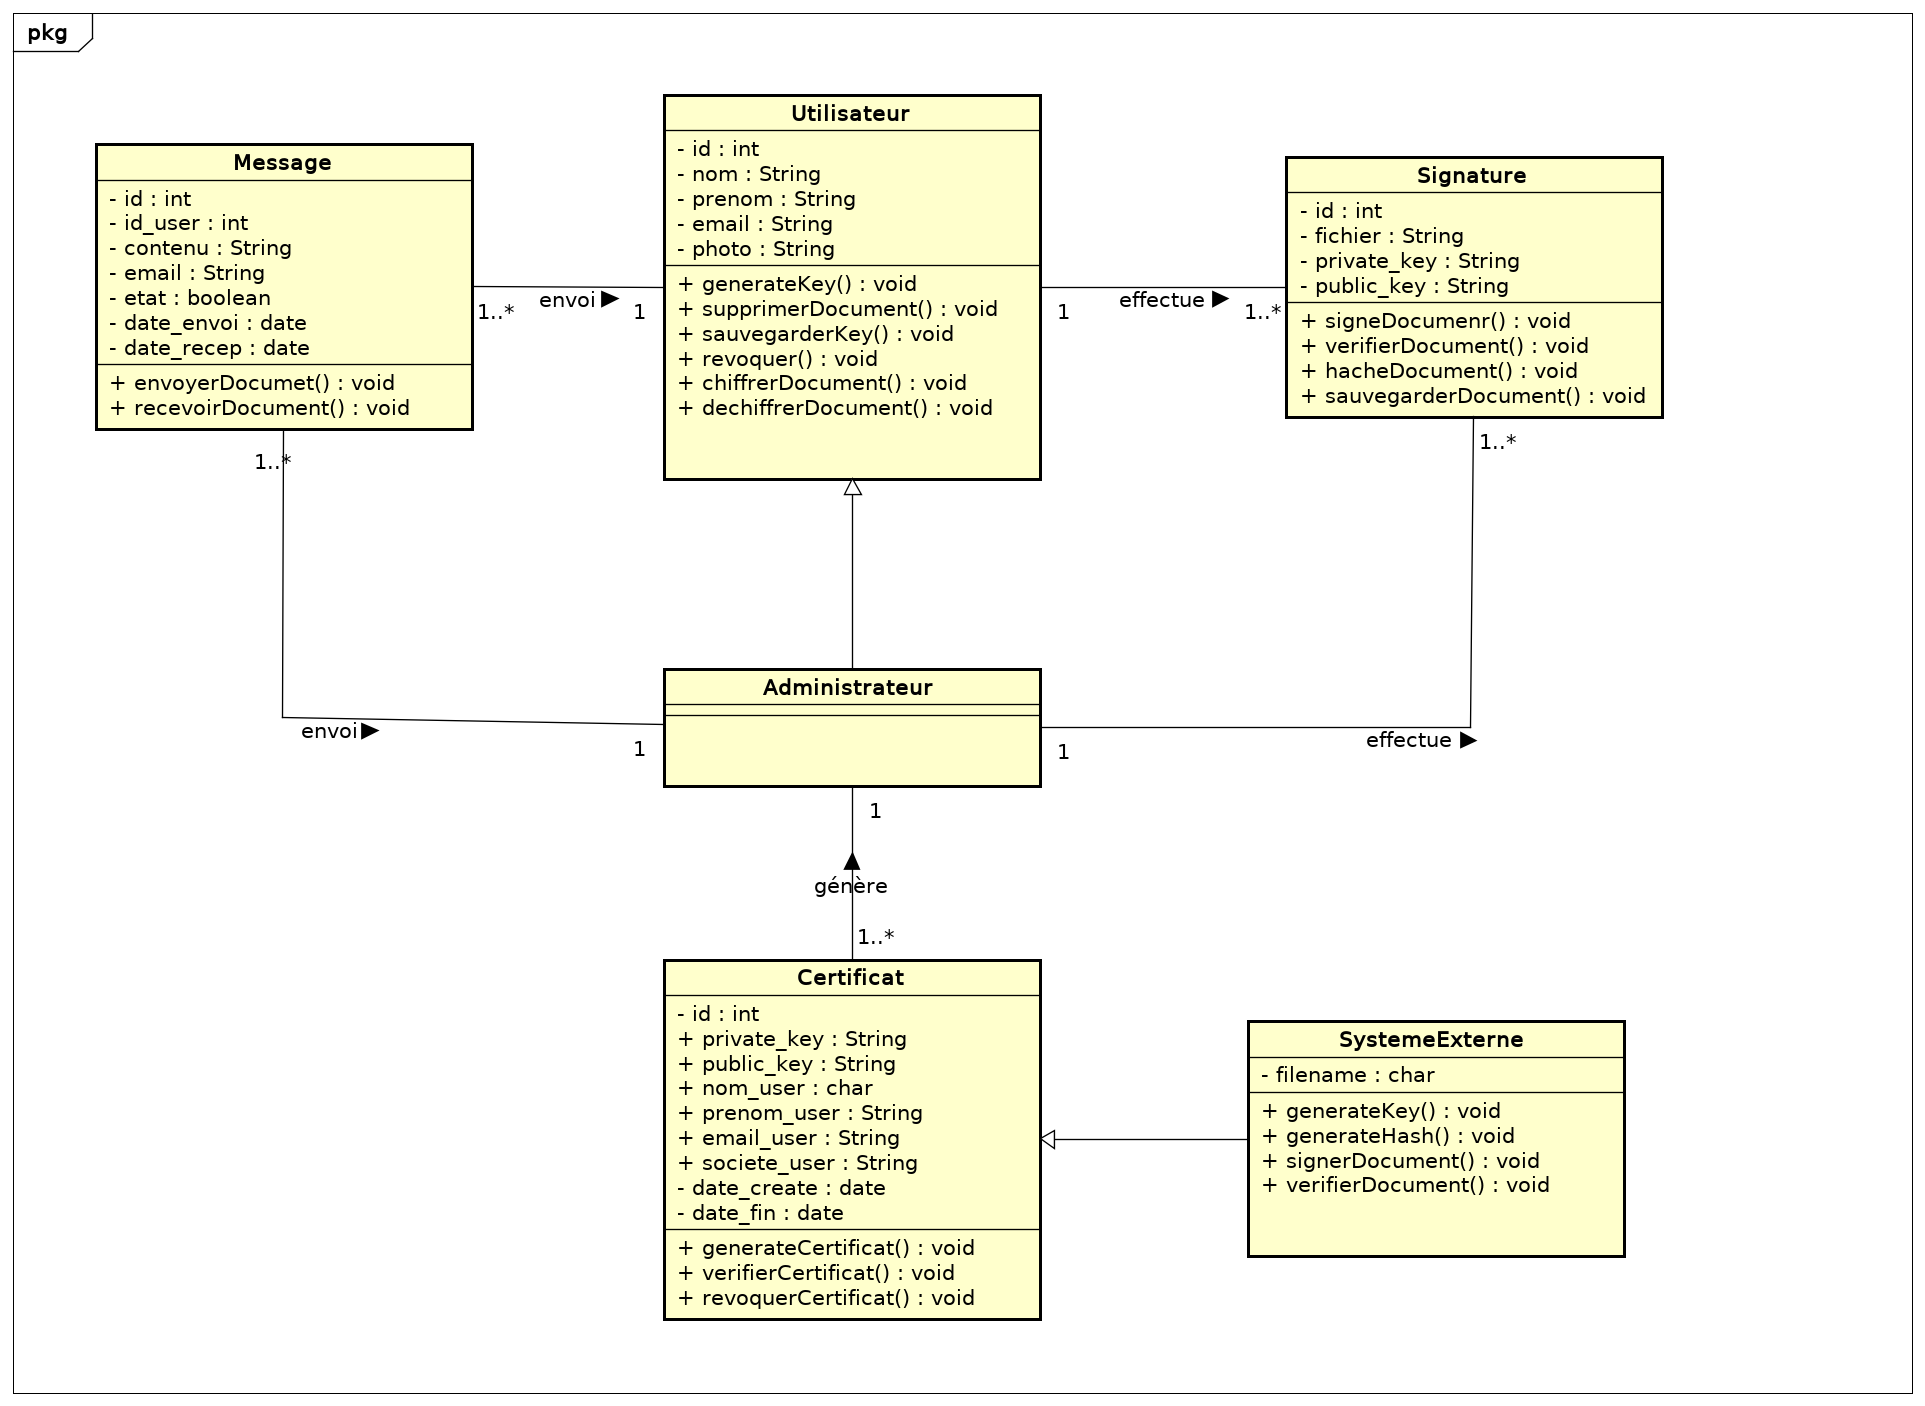
\includegraphics[width=18cm, height=13cm]{../Diagrammes/DigrammeClass/ClassDiagram.png}
					\caption{Diagramme de classe}
					\label{diaclass}
			\end{figure}	
			
			
		\subsubsection{Diagramme de packages}
		Lorsque nous sommes en présence d’un système de grande taille, il peut être intéressant de le décomposer en plusieurs parties (appelées paquetage).
Un paquetage est donc un regroupement de différents éléments d’un système (regroupement de
classes, diagrammes, fonctions, interfaces...). Cela permet de clarifier le modèle en l’organisant. Il est représenté par un dossier avec son nom à l’intérieur.
				\begin{figure}[H]
					\centering
					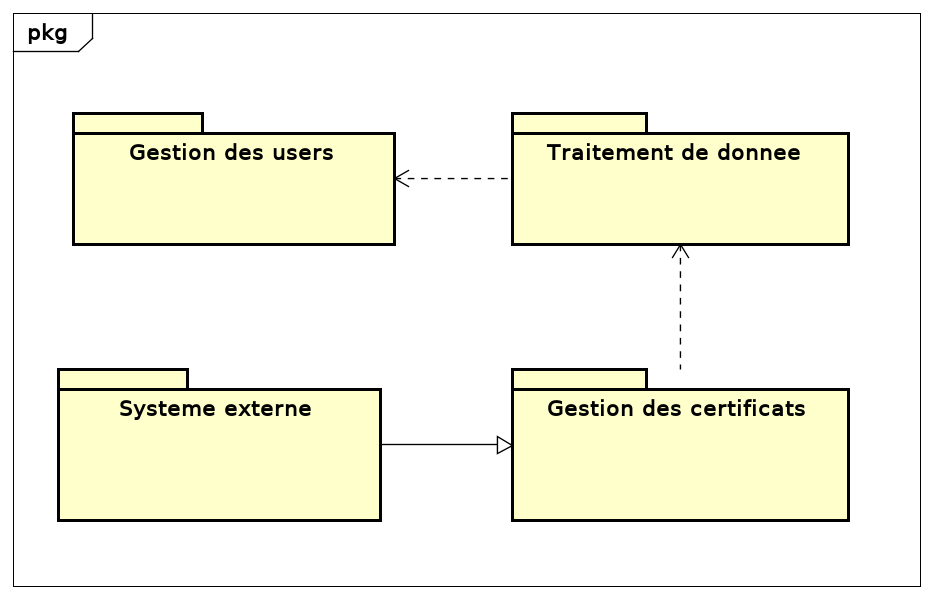
\includegraphics[width=18cm, height=13cm]{../Diagrammes/DigrammeClass/diagrammepackage.png}
					\caption{Diagramme de packages}
					\label{diapackage}
			\end{figure}
		
		\subsubsection{Diagramme de séquences}	
		 Pour décrire un scenario, UML propose un diagramme de séquences qui permet de décrire une séquence des messages échangés entre différents objets. Les diagrammes de séquences permettent de décrire comment les éléments du système interagissent entre eux et avec les acteurs. Les objets d'un système interagissent en s'échangeant des messages. Les acteurs interagissent avec le système au moyen d’interfaces homme-machine\cite{tatiana} .
		 \begin{enumerate}
		 	\item \textbf{Diagramme de séquence de cas d'utilisation s'authentifier :}
		 		\begin{figure}[H]
		 			\centering
		 			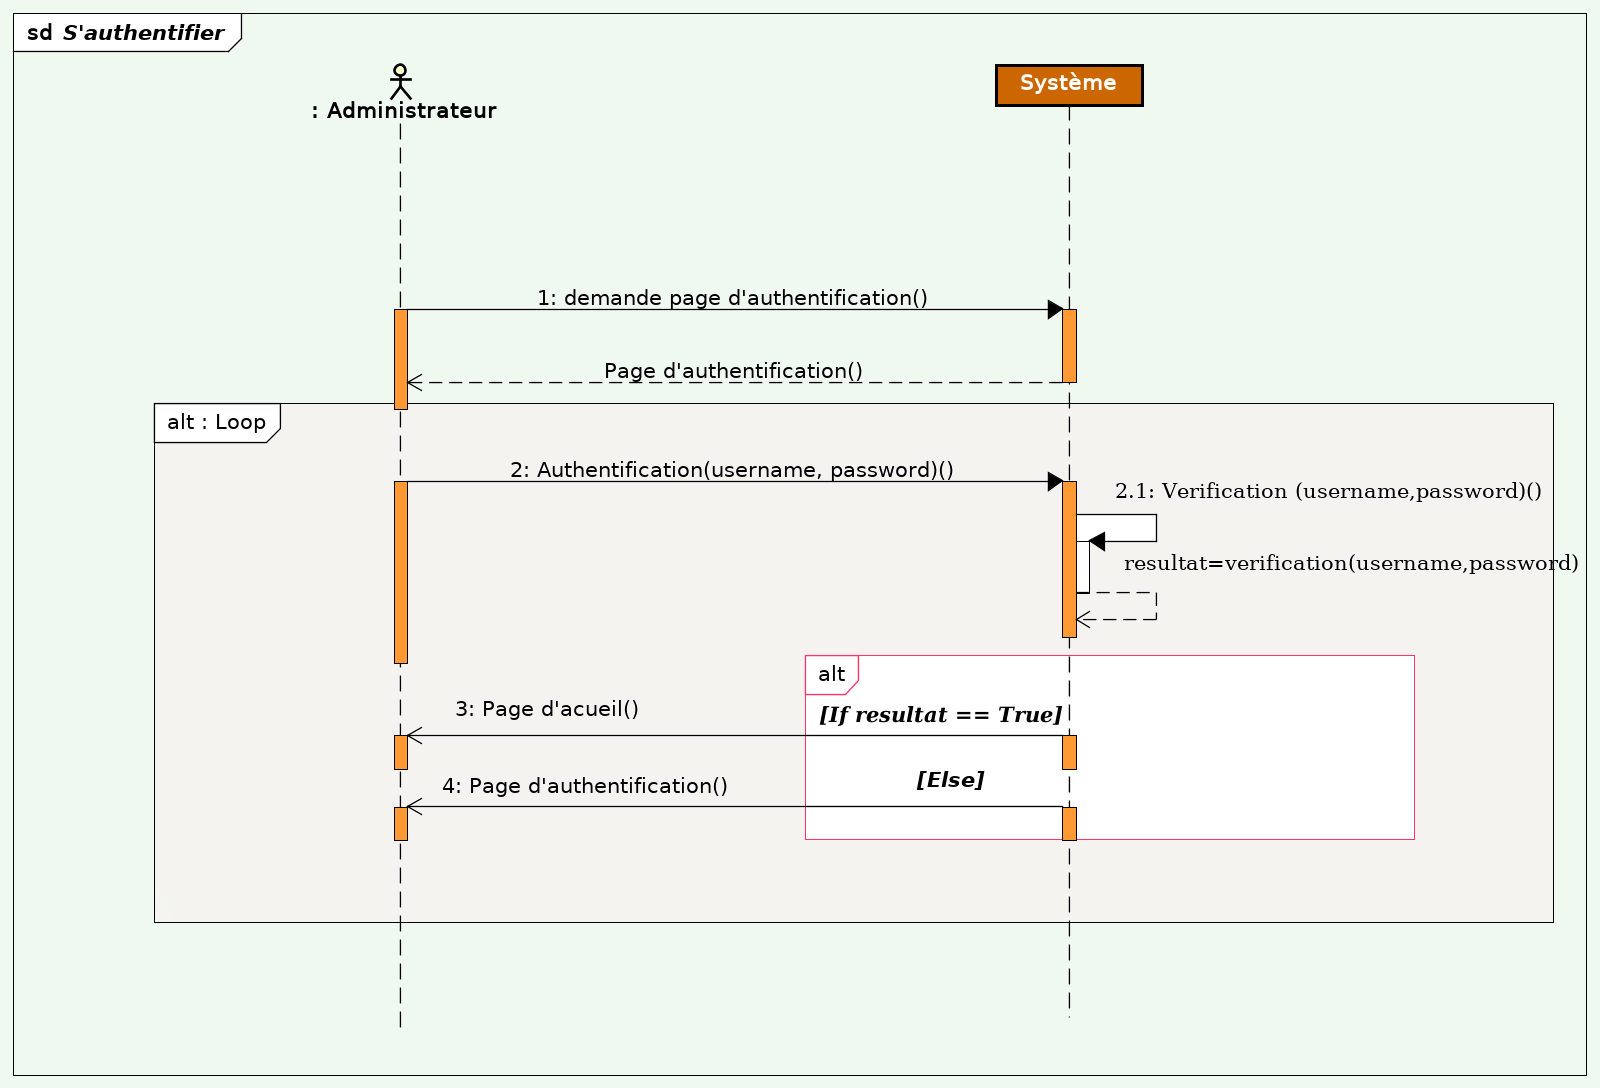
\includegraphics[width=17cm, height=11cm]{../Diagrammes/DiagrammeSequences/authentifiers.png}
		 			\caption{Diagramme de séquence de cas d'utilisation s'authentifier}
		 			\label{diaseq1}
		 		\end{figure}
		 		
		 	\item \textbf{Diagramme de séquence de cas d'utilisation générer key :}
		 	\begin{figure}[H]
		 		\centering
		 		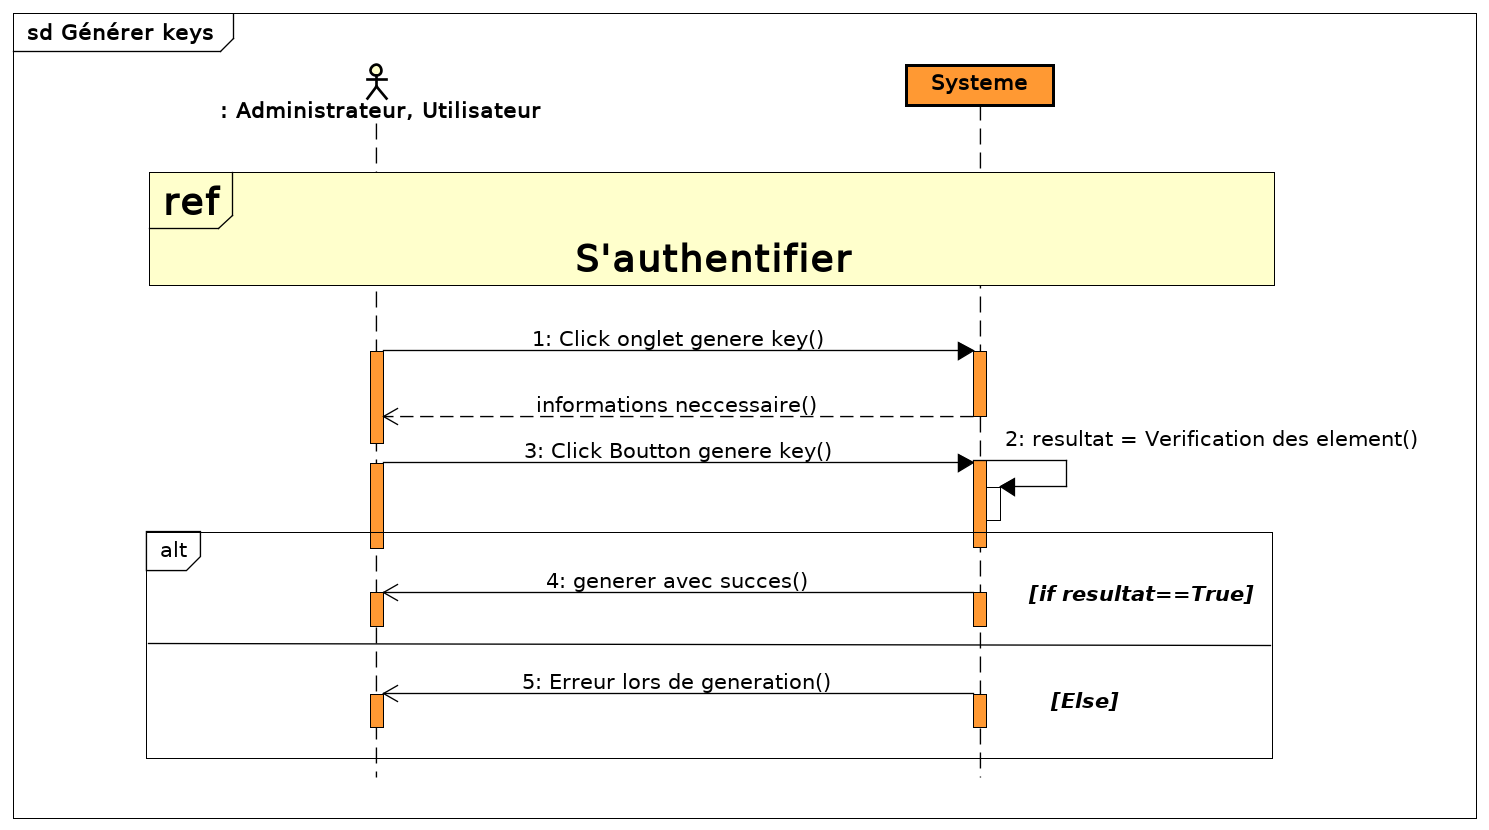
\includegraphics[width=18cm, height=13cm]{../Diagrammes/DiagrammeSequences/generatekeys.png}
		 		\caption{Diagramme de séquence de cas d'utilisation générer key}
		 		\label{diaseq2}
		 	\end{figure}
		 	
		 	\item Diagramme de séquence de cas d'utilisation certificat 
		 	\begin{figure}[H]
		 		\centering
		 		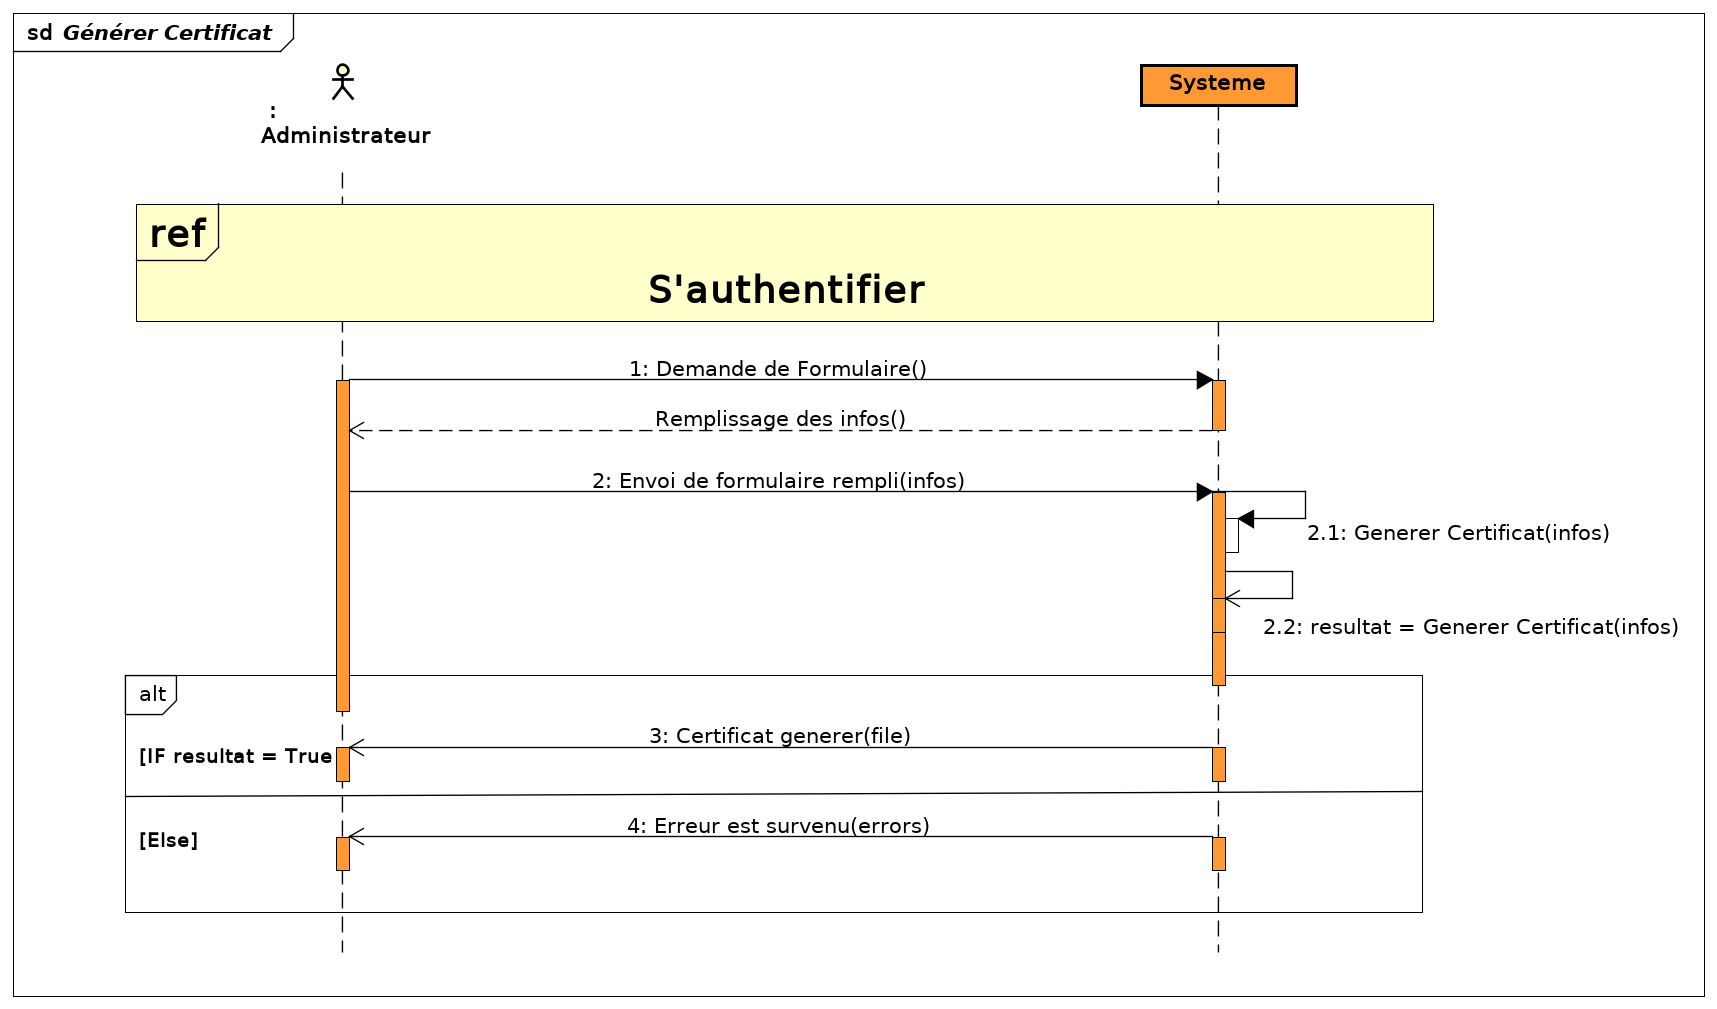
\includegraphics[width=18cm, height=13cm]{../Diagrammes/DiagrammeSequences/GenerateCertificat.png}
		 		\caption{Diagramme de séquence de cas d'utilisation générer certificat}
		 		\label{diaseq3}
		 	\end{figure}
		 	
		 	\item \textbf{Diagramme de séquence de cas d'utilisation signer document : }
		 	\begin{figure}[H]
		 		\centering
		 		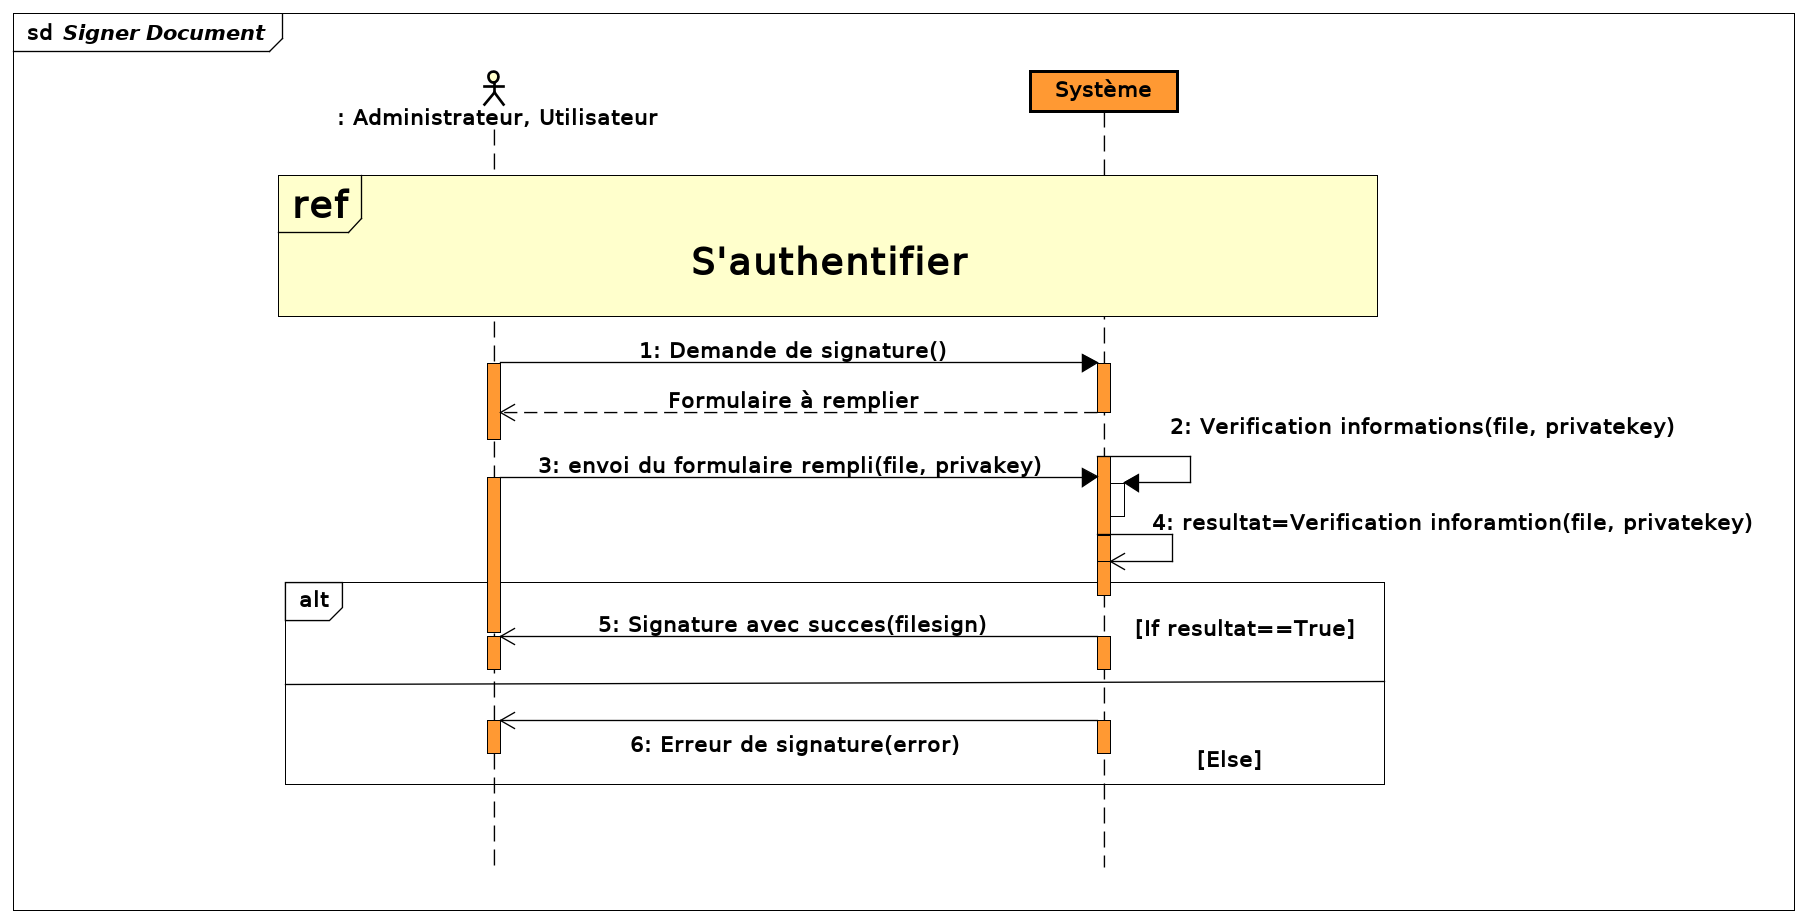
\includegraphics[width=18cm, height=13cm]{../Diagrammes/DiagrammeSequences/signerdocument.png}
		 		\caption{Diagramme de séquence de cas d'utilisation signer document}
		 		\label{diaseq4}
		 	\end{figure}
		 		
		 	\item \textbf{Diagramme de séquence de cas d'utilisation chiffrer/déchiffrer :}
		 	\begin{figure}[H]
		 		\centering
		 		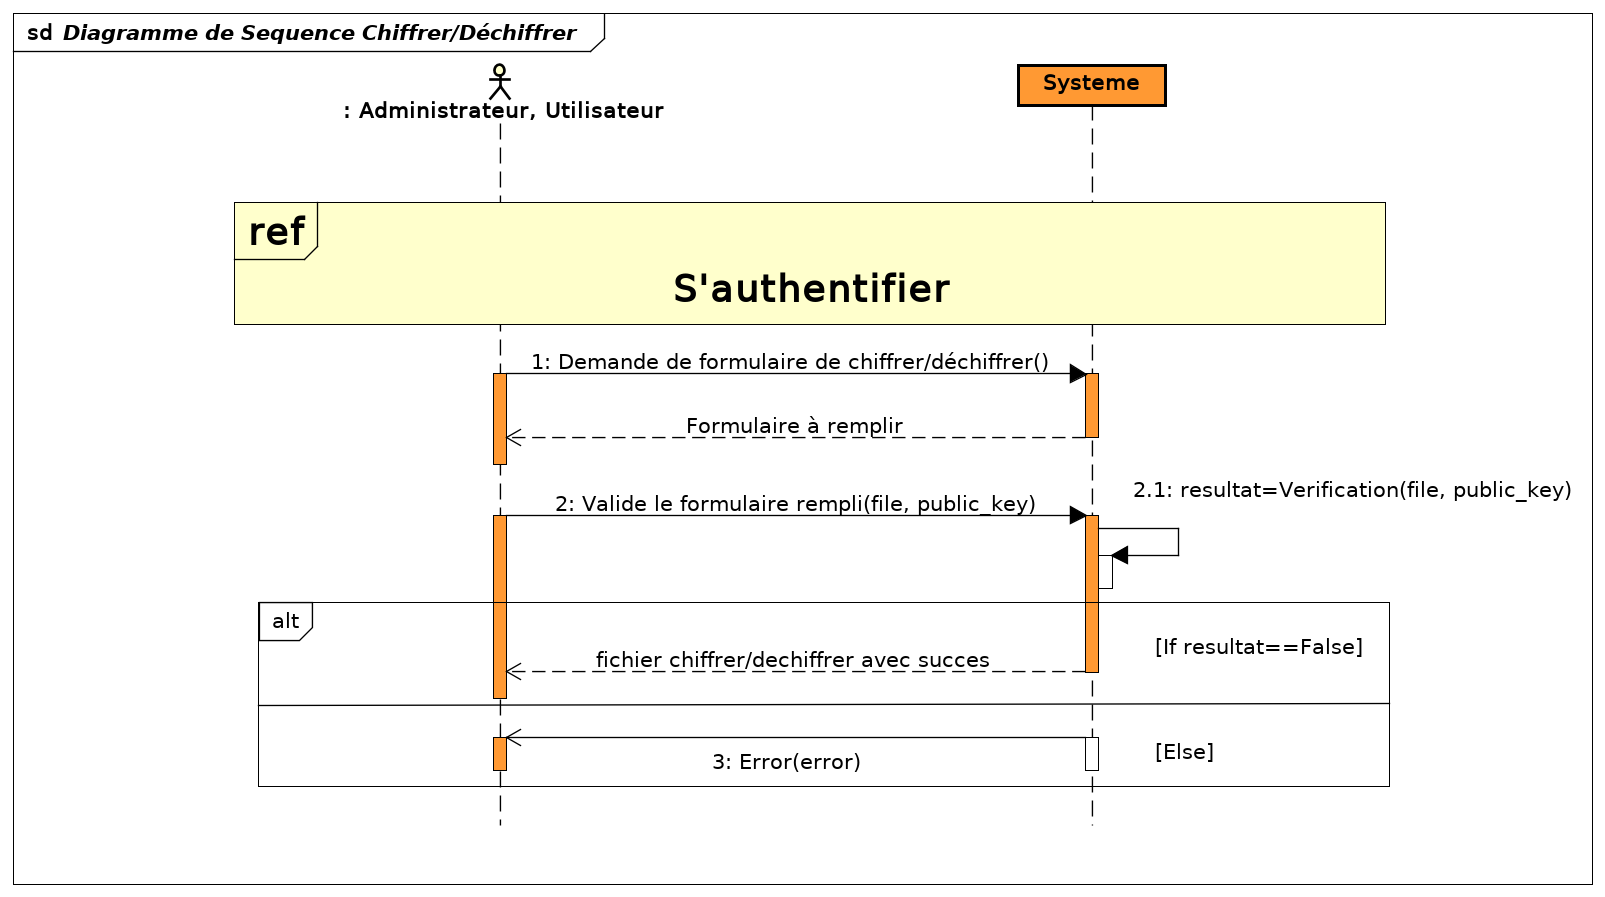
\includegraphics[width=18cm, height=13cm]{../Diagrammes/DiagrammeSequences/chiffrerDechiffrer.png}
		 		\caption{Diagramme de séquence de cas d'utilisation chiffrer/déchiffrer}
		 		\label{diaseq5}
		 	\end{figure}
		 	
		 	
		 		\item \textbf{Diagramme de séquence de cas d'utilisation envoyer document :}
		 	\begin{figure}[H]
		 		\centering
		 		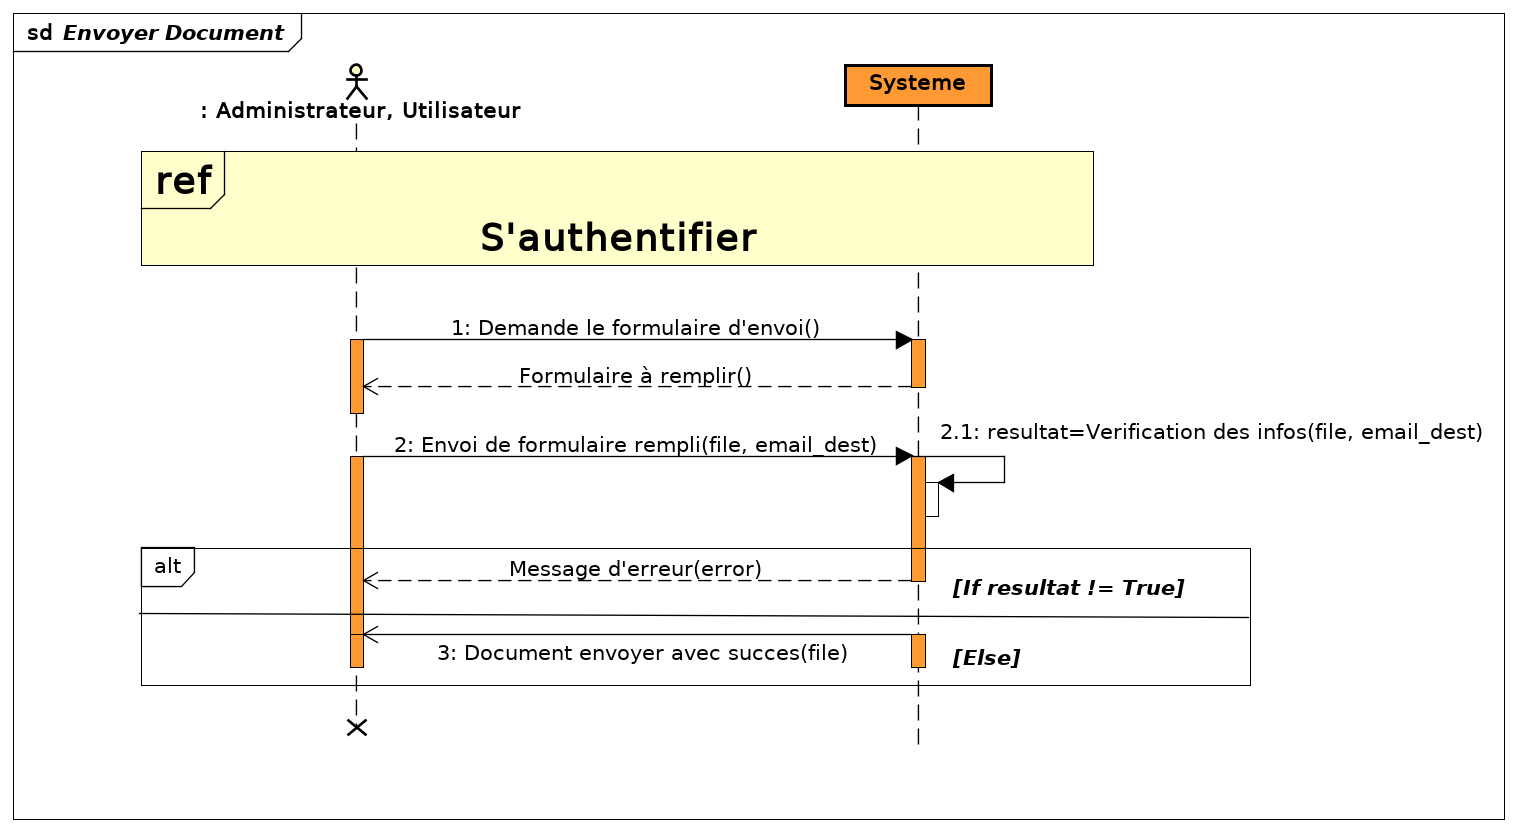
\includegraphics[width=18cm, height=13cm]{../Diagrammes/DiagrammeSequences/EnvoyerDocument.png}
		 		\caption{Diagramme de séquence de cas d'utilisation envoyer document}
		 		\label{diaseq6}
		 	\end{figure}
		 	
		 	
		 \end{enumerate}

		\subsubsection{Diagramme de déploiement}
	
			Dans le contexte du langage de modélisation unifié (UML), un diagramme de déploiement fait partie de la catégorie des diagrammes structurels, car il décrit un aspect du système même. Dans le cas présent, le diagramme de déploiement décrit le déploiement physique des informations générées par le logiciel sur des composants matériels. On appelle artefact l'information qui est générée par le logiciel\cite{deplymentid}.
			
		 	\begin{figure}[H]
		 		\centering
		 		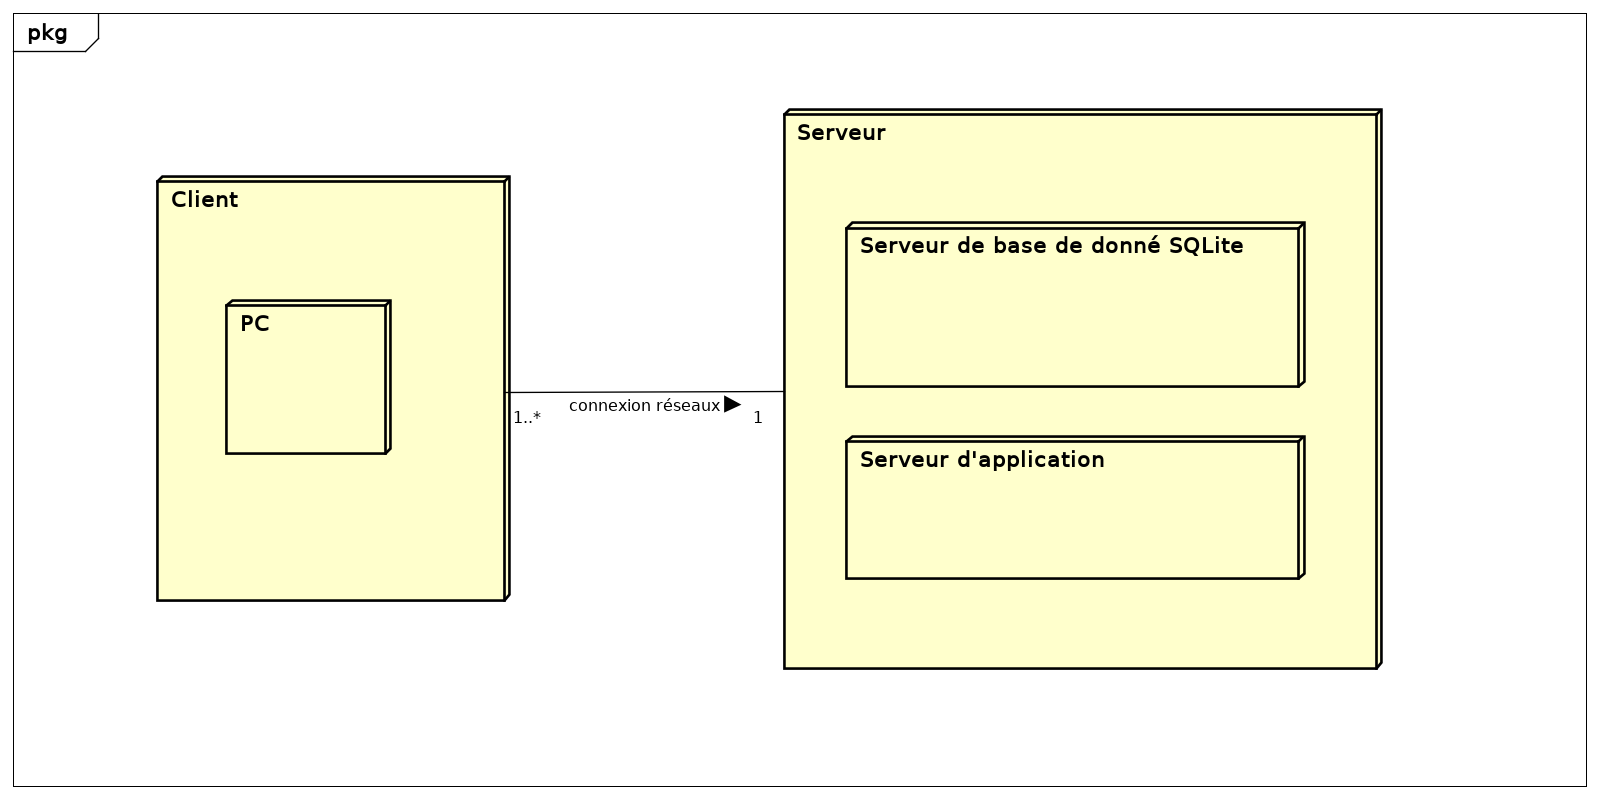
\includegraphics[width=17cm, height=11cm]{../Diagrammes/DiagrammeSequences/diagrammedeploy.png}
		 		\caption{Diagramme de séquence de cas d'utilisation envoyer document}
		 		\label{diadeploy}
		 	\end{figure}
		 	
			\subsubsection{Processus d'acquisition de certificat}
			Description...
		
		
	\section{Codage}
		\subsection{Environnement de développement}
		\subsection{Développement du module}
		\subsection{Développement de l'interface utilisateur}
	\section*{Conclusion}
	
	


%Chapitre 3
\chapter{RÉSULTATS ET COMMENTAIRES}
	\section*{Introduction}
		\lipsum[3]
	\section*{Conclusion}




\newpage
\addcontentsline{toc}{section}{Conclusion}
\section*{Conclusion}
%\end{flushleft}
\newpage
%\textbf{Ouvrages}
%\bibliographystyle{plain}
%\bibliography{biblnormecarte}
%\addcontentsline{toc}{section}{Référence Bibliographie}

			
\end{document}
